
%% 
%% Copyright 2007, 2008, 2009 Elsevier Ltd
%% F
%% This file is part of the 'Elsarticle Bundle'.
%% ---------------------------------------------
%% 
%% It may be distributed under the conditions of the LaTeX Project Public
%% License, either version 1.2 of this license or (at your option) any
%% later version.  The latest version of this license is in
%%    http://www.latex-project.org/lppl.txt
%% and version 1.2 or later is part of all distributions of LaTeX
%% version 1999/12/01 or later.
%% 
%% The list of all files belonging to the 'Elsarticle Bundle' is
%% given in the file `manifest.txt'.
%% 

%% Template article for Elsevier's document class `elsarticle'
%% with numbered style bibliographic references
%% SP 2008/03/01

\documentclass[preprint,12pt]{elsarticle}
%\documentclass[final,1p,times]{elsarticle}
\usepackage{lineno,hyperref}
\modulolinenumbers[5]

%\usepackage[notref]{showkeys}

%% Use the option review to obtain double line spacing
%% \documentclass[authoryear,preprint,review,12pt]{elsarticle}

%% Use the options 1p,twocolumn; 3p; 3p,twocolumn; 5p; or 5p,twocolumn
%% for a journal layout:
%% \documentclass[final,1p,times]{elsarticle}
%% \documentclass[final,1p,times,twocolumn]{elsarticle}
%% \documentclass[final,3p,times]{elsarticle}
%% \documentclass[final,3p,times,twocolumn]{elsarticle}
%% \documentclass[final,5p,times]{elsarticle}
%% \documentclass[final,5p,times,twocolumn]{elsarticle}

%% For including figures, graphicx.sty has been loaded in
%% elsarticle.cls. If you prefer to use the old commands
%% please give \usepackage{epsfig}

%% The amssymb package provides various useful mathematical symbols
\usepackage{amssymb}

\usepackage{amsmath}
\usepackage{amsfonts}
\usepackage{amssymb}
\usepackage{bm}
%% The amsthm package provides extended theorem environments
% %\usepackage{amsthm}

%% The lineno packages adds line numbers. Start line numbering with
%% \begin{linenumbers}, end it with \end{linenumbers}. Or switch it on
%% for the whole article with \linenumbers.
%% \usepackage{lineno}


\newtheorem{thm}{Theorem}
\newtheorem{lem}[thm]{Lemma}
\newdefinition{rmk}{Remark}
\newproof{pf}{Proof}
\newproof{pot}{Proof of Theorem \ref{thm2}}
\DeclareMathOperator*{\argmin}{arg\,min}

%\newtheorem{thm}{{\sc Theorem}}[section]
\newtheorem{dfn}{{\sc Definition}}[section]
\newtheorem{prp}{{\sc Proposition}}[section]
\newtheorem{lm}{{\sc Lemma}}[section]
\newtheorem{cor}{{\sc Corollary}}[section]
\newtheorem{ex}{{\sc Example}}[section]

%\journal{Reliability Engineering \& System Safety}

%% `Elsevier LaTeX' style
\bibliographystyle{elsarticle-num}
%%%%%%%%%%%%%%%%%%%%%%%

\begin{document}
\begin{frontmatter}


\title{TTT-SiZer: A graphic tool for aging trends recognition \tnoteref{title1}}

\author[inst1]{Maria Luz G\'amiz\corref{cor1}}
\ead{mgamiz@ugr.es}

\author[inst2]{Rafael Nozal-Ca\~nadas}
%\ead{}

\author[inst1]{Roc\'io Raya-Miranda}

\cortext[cor1]{Corresponding author}


\address[inst1]{Department of Statistics and O.R., University of Granada, Spain}
\address[inst2]{Department of Computer Science, UiT-The Arctic University of Norway , Norway}



\begin{abstract}
A new graphic tool is presented to test aging trends based on lifetime data.  The graphical test is developed by means of scale and space inference about the Total-Time-on-Test transform and its first and second derivatives. The graphic tool TTT-SiZer is defined considering nonparametric local polynomial kernel estimators and constructing the corresponding (simultaneous as well as punctual) confidence intervals around three different curves. The finite sample properties of the method are evaluated by a simulation study and the comparison with other non-graphical tests shows that the graphical test helps localize discrepancies of empirical data concerning a given hypothesized aging property, thus allowing to solve the problem locally. 
\end{abstract}

\begin{keyword}
Total-Time-on-Test Transform \sep Kernel smoothing \sep Order statistics \sep SiZer map
\MSC[2010] 90B25 \sep  62N05
\end{keyword}

\end{frontmatter}

\linenumbers

\section{Introduction}

In a technical context, aging is usually understood as a gradual decrease in performance over time, so it can be expected that the aging of a component or system increases the probability that it will fail. 

Let $X$ be the random variable that represents the lifetime of a mechanism. A natural measure of aging is the probability that $X$ exceeds a time $t + x$, assuming that the mechanism has an age of at least $t$. This idea leads to the concept of residual life. Also, the instantaneous propensity to the failure of a mechanism as a function of its age, that is, its failure rate, is a useful measure of aging. 
 
Aging trends evaluation of units and systems is a challenging subject in reliability and maintainability analysis and has attracted the attention of an increasing number of researchers. As a  result,  during the last years of the past century, different notions of aging  have given rise to a well-known nonparametric classification of life distributions,  which can be found among others in  \cite{BP75}, \cite{RH04}, and that remains a matter of interest, see for example \cite{KM2019}-\cite{KBM2020}  and references therein. In \cite{Lillo00} aging criteria based on the failure rate and mean residual life are considered, where it is analyzed whether a specific property of aging defined in terms of a reliability measure implies the same property or some other criterion is presented with another reliability measure. The monograph \cite{LX06}  provides an excellent revision and summary of the most widely studied aging concepts that are based on reliability characteristics such as the failure rate, the survival function or the mean residual life.  An exhaustive analysis of lifetime distributions in terms of their aging properties is presented.

Recently, new aging criteria have been mathematically formulated, see for example \cite{FPS2014}, \cite{NASS2014},  and \cite{Sz2018b}. They allow the analysis and measurement of the aging tendency from various points of view. Other approaches have  contributed to extending the mathematical formulation of aging in different application areas where the concept of failure rate, for example, is not so usual. In Chapter 4 of \cite{NSB2013}, the authors review some of the important results of the mathematical treatment of aging and translate the basic definitions to make them amenable for a quantile-based analysis. 

In this paper, the shape of the Total-Time-on-Test (TTT) curve is studied to figure out different types of aging of elements and systems. Our proposal is a useful and novel graphical tool that allows recognizing some important types of aging from empirical data.
The TTT plot was introduced  as a tool for analyzing failure data and some important classes of life distributions can be characterized in terms of the Total-Time-on-Test curve, see \cite{Klefsjo82}. 

The concept of TTT transform  has been extended and applied to different research fields, such as economics and actuarial sciences or biostatistics, see \cite{NS2013} and references therein for further details. In the field of reliability engineering the TTT curve has revealed as a very useful tool for aging characterization \cite{NS2013}, model identification \cite{Klefsjo82} and \cite{RH04},  hypothesis testing \cite{Klefsjo83a}, \cite{A1987},  stochastic ordering \cite{NSB2013}, age replacement policies in maintenance \cite{ZHMS2018}, structural reliability \cite{LS2019} , among others.  Recently \cite{NS2013} and \cite{FPS2014} have listed some known characterizations of common aging notions in terms of TTT function and have also derived some new ones. 

One of the advantages of the TTT curve is that it is confined to the compact interval $[0,1]$ whereas the failure rate is not bounded in general. Given the relationship between the failure rate and the TTT transform, one can understand the shape of the failure rate function by exploring the TTT curve. 
In this paper, the scaled TTT plot is used to discover a possible aging tendency of an underlying distribution based on sample information. In particular, increasing failure rate (IFR), bathtub failure rate (BFR) and new better than used in expectation (NBUE) are considered. \\
 
Identification of models by testing monotonic and non-monotonic trends has been a matter of research for decades in reliability and maintainability, \cite{KL98} and \cite{VV09}, where the property of non-aging can also be interpreted as the so-called ``as-good-as-new'' condition. In particular, the interest has traditionally been put on testing exponentiality against aging alternatives (see \cite{LX06} and \cite{Anis2013} for a detailed discussion) and it continues being a subject of study nowadays (\cite{SSA2018}, \cite{IM2019}, and \cite{CMO2019}). 

The contribution of this paper is twofold. On the one hand, a new estimator of the TTT-transform is proposed based on nonparametric statistics, more specifically, based on kernel smoothing techniques. To our knowledge, this is an innovative contribution to this area of Statistics. Although nonparametric smoothing techniques are very popular in related areas such as survival analysis, they are not very usual in reliability engineering where parametric methods have been traditionally preferred by the practitioners for solving inference problems. 
One motivation is the following. From available data, the theoretical TTT transform is usually approximated by means of the TTT-plot, the empirical estimator. While the theoretical curve is an absolutely continuous function, the empirical curve is always discontinuous and may be viewed as a poor approximation of the true curve, among other reasons, because it is a step function and the derivative either equals zero or is not defined, which makes difficult to evaluate shape characteristics. Kernel smoothing avoids discontinuities in the empirical function.

The second contribution is a new method for assessing non-aging properties in the underling lifetime. The new proposal is a graphical test able to recognize aging trends from data. The main advantage, compared to existing tests, is that it allows identifying specific areas where discrepancies from non-aging are detected. In contrast, standard testing methods summarize the sampling information in the single p-value to decide on the adequacy of the model specified in the null hypothesis.
%%%%%%%%%%%%%%%%%%%%%%%%%%%%%%%%%%%%%%%%%%%%%%%%%%%%%%%%%%%%%%%%%%%%%%%%%%%%%%%%%%%%%%%%%%%%%%%%%%%

The paper is organized as follows. In Section 2 the Total-Time-on-Test transform is formally defined and some relevant properties are reviewed. Section 3 introduces local-polynomial estimators for the TTT-curve and its two first derivatives. Section 4 is devoted to SiZer map methodology. 
 
A graphical method for hypothesis testing is proposed. The good performance of the new graphical test is evaluated by an extensive simulation study and the method is applied to several real datasets in Section 5. Conclusions and future research interests are summarized in Section 6. Finally, some mathematical developments are included in the Appendix.
%%%%%%%%%%%%%%%%%%%%%%%%%%%%%%%%%%%%%%%%%%%%%%%%%%%%%%%%%%%%%%%%%%%%%%%%%%%%%

\section{Preliminary}\label{sec:pre}
In this section some notation is fixed and the concepts needed for the rest of the paper are defined.

\subsection{Reliability classes based on aging notions}
Let $X$ denote a random lifetime with absolutely continuous distribution function, with survival function $S$, for any fixed $t>0$ let $X_t$ denote the \textit{residual lifetime} from time $t$, that is, the additional lifetime from $t$. The conditional survival function, given that $T>t$ is  $S_t(x)=S(t+x)/S(t)$, for all $x >0$. The mean residual time is then defined as $\mu_t= \int_0^{+\infty} \frac{S(t+x)}{S(t)}dx$. Note that $\mu_0=E[X]=\mu$. For a continuous random variable $X$, with density $f$, and survival function $S$, the corresponding \textit{failure rate} or \textit{hazard function} is defined as $h(t)=f(t)/S(t)$.

\begin{enumerate}
\item Increasing failure rate, $IFR$:\\
\noindent $X$ is {\it IFR}, if and only if, for all $x>0 $ fixed, $S_{t_1}(x) \leq S_{t_2}(x)$,  and for all $t_1 < t_2$. Equivalently, $X$ is {\it IFR} if and only if $h(t)$ is increasing  in $t$.

\item Bathtub shaped Failure Rate, $BFR$:\\
\noindent $X$ is  {\it BFR}, if and only if, its  failure rate curve is divided into three regions: decreasing failure rate region, constant failure rate region, and increasing failure rate region.



\item New better than used in expectation, $NBUE$:\\
 \noindent $X$  is {\it NBUE}, if and only if,  $\mu_t \leq  \mu$, for all $t>0$.

\end{enumerate}


\subsection{Total-Time-on-Test transform: Definition and relevant properties} \label{sec:TTT}
In reliability essays, when several units are tested for studying their life lengths some of the units would fail while others may survive the test period. The sum of all observed and incomplete life lengths is the total time on test statistics. The plot of this statistic versus time is called the total-time-on-test plot. As the number of units on a test tends to infinity the limit of this statistic is called the total time on test transform (TTT). 

\begin{dfn} \textbf{Total-Time-on-Test statistic}: \label{ttt.def1}
\noindent Suppose $n$ items under test and successive failures are observed at $0=X_{(0)} \leq X_{(1)} \leq X_{(2)}\leq \cdots \leq X_{(n)}$, with $X_{(i)}$ the $i$-th order statistic from a lifetime random variable $X$ with absolutely continuous distribution function $F$. Then the \textit{total time on test statistic} during the interval $(0,t)$ is defined as 
\[
\tau (t) = \sum_{i=1}^r X_{(i)}+\left(n-r\right)t,
\]
provided that $X_{(r-1)}<t\leq X_{(r)}$.
\end{dfn}

%%%%

\begin{dfn}\textbf{Total Time on Test transform}: \label{ttt.def2} 
\noindent Let $X$ be a (non-negative) random variable with absolutely continuous cumulative distribution function $F$. The \textit{total time on test transform} of $X$ is defined as
\begin{equation} \label{ttt.curve}
\varphi(p) =\displaystyle{\int_0^{Q(p)}}\left(1-F(t)\right) dt,
\end{equation}
where $Q(p)= F^{-1}(p)$, for $p\in [0,1]$ denotes the corresponding quantile function.
\end{dfn}
When $E[X]=\mu < \infty$, it can be seen that $\mu=\int_0^{Q(1)} S(t)dt$. The {\textit{scaled}} TTT transform is then defined as $\varphi(p)/\mu$, for $0 \leq p \leq 1$,  which is scale-invariant. In the following, the notation $\varphi(p)$ is kept for the scaled TTT transform, and it is assumed that $\mu=1$ since it does not imply any loss of generality.


\subsection{Aging properties based on the TTT transform}\label{sec:aging}
%

The TTT plot is used as a tool for model selection. Thus, when the TTT plot produces a cloud of points around the diagonal of the square  unit, the exponential distribution fits well of the underlying lifetime $F$, since $\varphi_{Exp}(p)=p$, for $0 \leq p \leq 1$. 

Other failure rate shapes can be recognized from an inspection of the TTT plot. A convex TTT curve corresponds with a decreasing failure rate (DFR); a concave TTT curve corresponds with an increasing failure rate (IFR). When the TTT plot describes a trajectory first convex and then concave it indicates a bathtub failure rate shape and when it is first concave and then convex, it indicates a unimodal failure rate shape. 

Let $X$ be a lifetime with distribution function $F$ and with finite mean $\mu$. 

\begin{prp} {TTT-curve characterization of aging} \

\begin{enumerate}
\item $ F$ is $ IFR$, if and only if, $ \varphi'' (u) \leq  0$, for all $0 <u <1$;
\item $F$ is $BFR$, if and only if, for some $u_0 \in (0,1)$, $\varphi'' (u) (u-u_0) >0 $, for all $0 <u <1$;
\item $F$ is $ NBUE$, if and only if, $\varphi(u)/u \geq  1$, for all $0 <u <1$.
\end{enumerate}
 \end{prp}

Thus, one of the main objectives of this paper is to estimate TTT-curve as well as  the first and second derivatives to search for aging trends.
%%%%%%%%%%%%%%%%%%%%%%%%%%%%%%%%%%%%%%%%%%%%%%%%%%%%%%%%%%%%%%%%%%%%%%%%%%%%%
%%%%%%%%%%%%%%%%%%%%%%%%%%%%%%%%%%%%%%%%%%%%%%%%%%%%%%%%%%%%%%%%%%%%%%%%%%%%%

%
\section{Local polynomial estimation of the TTT-transform and its first and second derivatives}\label{locpol}
In this section  a local-polynomial estimator for the TTT-transform directly formulated from an empirical estimation of the TTT-curve is suggested, that is, there is no need to estimate the quantiles to get an estimator of the TTT-transform.

%
\subsection{Least-squares estimation of the Total-Time-on-Test transform}

Let $X_1,X_2,\cdots,X_n$ be an independent and identically distributed random sample drawn form an absolutely continuous distribution function $F$ with density $f$. Let $X_{(1)},X_{(2)},\ldots,X_{(n)}$ denote the corresponding order statistics. Let us denote $p_i=\frac{i}{n}$ for $i= 1,2, \ldots, n$. An empirical ($naive$) estimator of the TTT-curve $\widehat{\varphi}_{n,i}$, can be defined as follows
%
\begin{equation}\label{empi}
\widehat{\varphi}_{n,i}= \sum_{j=1}^i \left(1-\frac{j-1}{n}\right) \left(X_{(j)}-X_{(j-1)}\right),
\end{equation}
for $i=1,2,\ldots,n$, with $\widehat{\varphi}_{n,0}=0$. As can be seen $\widehat{\varphi}_{n,n}=\bar{X}$, the mean sample statistics. Since the properties of the curve are not affected by scale changes, the curve can be confined to the interval $[0,1]$ by first normalizing the data. In the following, without loss of generality, it is assumed that $\bar{X}=1$.

Under a local-polynomial approach, for each estimation point $p_0 \in (0,1)$, the TTT-transform $\varphi(p_0)$ is locally (in a neighborhood of $p_0$) approximated by a $m$th-degree polynomial function in the sense that for all $p \in \left(p_0-h,p_0+h\right)$ it holds that $\varphi(p)=\theta_0+\theta_1(p-p_0)+\theta_2(p-p_0)^2+\ldots+\theta_m(p-p_0)^m$, for an appropriate bandwidth $h$. 

The parameters of the model can be interpreted respectively as $\theta_0={\varphi}(p_0)$; ${\theta}_1={\varphi'}(p_0)$; and, in general, ${\theta}_k=\frac{\varphi^{(k)}(p_0)}{k!}$, for $k=1,2,\ldots,m$. The approximation above is valid locally if certain smoothness conditions on the true curve, in the sense of derivability, are assumed. 

In particular, the three first coefficients provide the following estimates: $\widehat{\varphi}(p_0)=\widehat{\theta}$, $\widehat{\varphi}'(p_0)=\widehat{\theta}_1$, and $\widehat{\varphi}''(p_0)=2\widehat{\theta}_2$, respectively.
To this goal, the following least-squares problem is formulated.

\begin{eqnarray}\label{LS}
&&\left(\widehat{\theta}_0,\widehat{\theta}_1,\ldots,\widehat{\theta}_m\right)^{\intercal}= \\
\nonumber &&\underset{\left({\theta}_0,\theta_1,\ldots, {\theta}_m\right)^{\intercal}}{\arg \min} \sum_{i=1}^n\left\{\widehat{\varphi}_{n,i}-\theta_0-\theta_1(p_i-p_0)-\ldots-\theta_m(p_i-p_0)^m\right\}^2 K_h(p_i-p_0),
\end{eqnarray}
where $K_h(\cdot)=\frac{1}{h}K(\frac{\cdot}{h})$, with $K$ a symmetric kernel function, and $h$ the bandwidth parameter that controls the size of the window around the estimation point, $p_0$, where the polynomial approximation is valid.
After differentiating in equation ($\ref{LS}$), for $m=2$ with respect to $\theta_j$ ($j=0, 1, 2$), it is obtained a system of linear equations that can be written in matrix form
\begin{equation}\label{score}
\left(\begin{array}{cccc}
a_0 & a_1&\cdots &a_m \\ 
a_{1} & a_2&\cdots &a_{m+1}\\
\vdots & \vdots &\ddots &\vdots \\ 
a_m & a_{m+1}&\cdots &a_{2 m} 
\end{array}\right)
\left(\begin{array}{c}
 \theta_0 \\ 
\theta_1 \\ 
\vdots \\
\theta_m
 \end{array}\right)=
\left(\begin{array}{c} 
A_0 \\ 
A_1 \\ 
\vdots \\
A_m
 \end{array}\right);
\end{equation}
where 
\begin{equation}\label{bigA}
A_r(p_0)=\sum_{i=1}^n (p_i-p_0)^r K_h(p_i-p_0)\widehat{\varphi}_{n,i}, \ \ r=0,1,\ldots,m;
\end{equation}
and 
\begin{equation}\label{smallA}
a_l(p_0)=\sum_{i=1}^n(p_i-p_0)^l K_h(p_i-p_0), \ \ l=0,1,2,\ldots,2m.
\end{equation}

In \cite{ZHMS2018} the authors also consider a least-squares optimization problem based on the TTT-plot. They assume a Weibull model and, from a dataset, they estimate the shape parameter by minimizing the distance between the TTT-plot and the TTT-transform of the Weibull model. In this paper, a more general and versatile approach is considered, that is, the optimization problem is formulated assuming no specific parametric form for the theoretical TTT-transform.


\subsection{Local-quadratic estimator}\label{quad}
For illustrative purposes, in the following, the data are fit locally using a 2-degree polynomial. However, it should be taken into account that it is convenient to increase the complexity of the model when interested in exploring the properties of the form through the second derivative. Detailed expressions for the estimators based on a local-cubic polynomial fit are given in \ref{ap:cubic}.

The least-squares problem  ($\ref{LS}$) is set for $m=2$, and $A_r(p_0)$ are defined as in \eqref{bigA} for $ r=0,1,2$; and  $
a_l(p_0)$, for $ l=0, 1, 2, 3, 4$ as in \eqref{smallA}. The estimator of the TTT-transform is denoted $\widehat{\varphi}_{h}(\cdot)$. 


The Cramer's rule provides an appropriate solution to the equations that leads to the estimation of the curve $\varphi$ and its derivatives at a given $p_0$, based on the quadratic fit as follows.

\begin{itemize}
\item { The TTT-curve}
\begin{equation}\label{theta0}
\widehat{\varphi}_{h}(p_0)= \widehat{\theta}_0(p_0)= \sum_{i=1}^n \bar{{K}}_{0,h}\left(p_i-p_0\right) \widehat{\varphi}_{n,i},
\end{equation}
where
\begin{eqnarray*}
\hskip-1cm &&\bar{{K}}_{0,h}\left(p_i-p_0\right)=\\
\hskip-1cm &&\frac{\left(a_1a_3-a_2^2\right)\left(p_i-p_0\right)^2+\left(a_2a_3-a_1a_4\right)\left(p_i-p_0\right)+\left(a_2a_4-a_3^2\right)}{a_0a_2a_4+2a_1a_2a_3-a_2^3-a_0a_3^2-a_1^2a_4} K_h\left(p_i-p_0\right).
\end{eqnarray*}

\item{The first derivative}
\begin{equation}\label{theta1}
\widehat{\varphi}'_{h}(p_0)=\widehat{\theta}_1(p_0)= \sum_{i=1}^n \bar{{K}}_{1,h}\left(p_i-p_0\right) \widehat{\varphi}_{n,i},
\end{equation}
where 
\begin{eqnarray*}
\hskip-1cm &&\bar{{K}}_{1,h}\left(p_i-p_0\right)= \\
\hskip-1cm &&\frac{\left(a_1a_2-a_0a_3\right)\left(p_i-p_0\right)^2+\left(a_0a_4-a_2^2\right)\left(p_i-p_0\right)+\left(a_2a_3-a_1a_4\right)}{a_0a_2a_4+2a_1a_2a_3-a_2^3-a_0a_3^2-a_1^2a_4} K_h\left(p_i-p_0\right).
\end{eqnarray*}

\item{ The second derivative }

\begin{equation}\label{theta2}
\widehat{\varphi}''_h(p_0)=2 \widehat{\theta}_2(p_0) =2 \sum_{i=1}^n \bar{{K}}_{2,h}\left(p_i-p_0\right) \widehat{\varphi}_{n,i}
\end{equation}
where 
\begin{eqnarray*}
\hskip-1cm &&\bar{{K}}_{2,h}\left(p_i-p_0\right)=\\
\hskip-1cm &&\frac{\left(a_0a_2-a_1^2\right)\left(p_i-p_0\right)^2+\left(a_1a_2-a_0a_3\right)\left(p_i-p_0\right)+\left(a_1a_3-a_2^2\right)}{a_0a_2a_4+2a_1a_2a_3-a_2^3-a_0a_3^2-a_1^2a_4} K_h\left(p_i-p_0\right).
\end{eqnarray*}
\end{itemize}

%\bigskip
%%%%%%%%%%%%%%%%%%%%%%%%%%%%%%%%%%%%%%%%%%%%%%%%%%%
%%%%%%%%%%%%%%%%%%%%%%%%%%%%%%%%%%%%%%%%%%%%%%%%%%%

\subsection{Statistical properties of the estimator}\label{stat_prop}
This section is devoted to the local-quadratic case. Similar results for the local-cubic estimator can be derived and are sketched in \ref{ap:cubic}.

The SiZer methodology involves the construction of confidence intervals around the target function and then it is needed to derive statistical properties such as mean and variance. First, expressions in \eqref{theta0}-\eqref{theta2} are rewritten as a linear combination of the order statistics $X_{(1)} \leq X_{(2)} \leq \cdots \leq X_{(n)}$ so that each estimator is written in terms of the corresponding $L$-estimator. Then, in \ref{apx:moments} the results in \cite{HE2000} help to obtain exact analytic expressions for the bootstrap moments.
 
The empirical estimator $\widehat{\varphi}_{n,i}$ ($i=1,\ldots,n$) given in ($\ref{empi}$) can be expressed as
\begin{equation}\label{empi_2}
\widehat{\varphi}_{n,i}=\sum_{j=1}^i\omega_{i,j} X_{(j)},
\end{equation}
where
\begin{equation}\label{eq:omega}
\omega_{i,j}=\left\{\begin{array}{cll} 
\frac{1}{n}, & \hspace{0.3cm}& j= 1,2, \ldots, i-1; \\
\frac{n-(i-1)}{n},& \hspace{0.3cm}& j= i. \\
\end{array}\right.
\end{equation}
These weights can be arranged in matrix form  as 
\[
{\bf W} =\left(
\begin{array}{cccccc}
1 & 0 &0 &0& \cdots &0 \\
\frac{1}{n} & \frac{n-1}{n}&0&0&\cdots& 0 \\
\frac{1}{n} & \frac{1}{n}&\frac{n-2}{n}&0&\cdots& 0 \\
\frac{1}{n} & \frac{1}{n}&\frac{1}{n}&\frac{n-3}{n}&\cdots& 0 \\
\vdots&\vdots&\vdots&\vdots&\vdots&\vdots \\
\frac{1}{n} & \frac{1}{n}&\frac{1}{n}&\cdots&\frac{1}{n}& \frac{1}{n} \\
\end{array}
\right).
\]


Expressions for the estimators of the TTT-transform and its derivatives as L-estimators can be obtained. 
\noindent Equations \eqref{empi_2} and  \eqref{theta0} lead to
\begin{eqnarray*}
\widehat{\varphi}_h(p_0)&=&\sum_{i=1}^n \bar{K}_{0,h}(p_i-p_0)\sum_{j=1}^i\omega_{i,j}X_{(j)}= \\
&=& \sum_{i=1}^n \sum_{j=1}^i \bar{K}_{0,h}(p_i-p_0)\omega_{i,j}X_{(j)}, 
\end{eqnarray*}
and, re-ordering the terms inside the sums, 
\begin{equation}%\label{L.estim1}
\widehat{\varphi}_h(p_0)=  \sum_{j=1}^n \sum_{i=j}^n \bar{K}_{0,h}(p_i-p_0)\omega_{i,j}X_{(j)}. 
\end{equation}
Using matrix notation the above expression can be written as
\begin{equation}\label{L.estim1}
\widehat{\varphi}_h(p_0)=  \bar{\bf K}_{0,h}(p_0)^{\intercal} \cdot {\bf W} \cdot{\bf X}_{(\cdot)}, 
\end{equation}
where the vector of weights is denoted
$$\bar{\bf K}_{0,h}(p_0)=\left(\bar{K}_{0,h}(p_1-p_0), \bar{K}_{0,h}(p_2-p_0),\ldots,\bar{ K}_{0,h}(p_n-p_0)\right)^{\intercal},$$ and ${\bf X}_{(\cdot)}=\left(X_{(1)},\ldots,X_{(n)}\right)^{\intercal}$ is the ordered sample. 
%

\vskip0.3cm

Let us introduce the following notation
\begin{equation}\label{mean}
\boldsymbol{\mu}=\left({\mu}_{(1)},{\mu}_{(2)},\ldots,{\mu}_{(n)}\right)^{\intercal}, 
\end{equation}
with $\mu_{(i)}=E\left[X_{(i)}\right]$, for $i=1,2,\ldots,n$, is the vector of means of the order statistics;  and,  
\begin{equation}\label{var}
{\boldsymbol{\Sigma}}=\left(\begin{array}{cccc}
\sigma_{(1)}^2 & \sigma_{(12)} & \cdots & \sigma_{(1n)} \\
\sigma_{(12)} & \sigma_{(2)}^2 & \cdots & \sigma_{(2n)} \\
\vdots & \vdots & \ddots & \vdots \\
\sigma_{(1n)} & \sigma_{(2n)} & \cdots & \sigma_{(n)}^2
\end{array}\right),
\end{equation}
with $\sigma_{(i)}^2={\rm Var}(X_{(i)})$ and $\sigma_{(ij)}={\rm Cov} \left(X_{(i)},X_{(j)} \right)=E\left[\left(X_{(i)}-\mu_{(i)}\right)\cdot\left(X_{(j)}-\mu_{(j)} \right)\right]$, for $i, j= 1,2,\ldots,n$, $i<j$, is the covariance matrix. 

Then, the variance of the estimator of the TTT-transform can be computed by
\begin{equation}\label{V.phi0}
{\rm Var} \left(\widehat{\varphi}_h(p_0)\right)= \bar{\bf K}_{0,h}(p_0)^{\intercal}\cdot {\bf W} \cdot {\boldsymbol{\Sigma}}\cdot  {\bf W}^{\intercal}\cdot \bar{\bf K}_{0,h}(p_0).
\end{equation}


%\subsubsection*{The first derivative of the TTT-transform}
\noindent Similar to \eqref{V.phi0}  the corresponding expression for the first derivative of the TTT-curve can be obtained. Let us define the corresponding vector of weights 
$$\bar{\bf K}_{1,h}(p_0)=\left(\bar{ K}_{1,h}(p_1-p_0), \bar{ K}_{1,h}(p_2-p_0),\ldots,\bar{ K}_{1,h}(p_n-p_0)\right)^{\intercal},$$ 
then it can be written
\begin{equation*}
\widehat{\varphi}'_h(p_0)=  \sum_{j=1}^n \sum_{i=j}^n \bar{K}_{1,h}(p_i-p_0)\omega_{i,j}X_{(j)}=\bar{\bf K}_{1,h}(p_0)^{\intercal} \cdot {\bf W} \cdot{\bf X}_{(\cdot)}, 
\end{equation*}
and the variance is given as
\begin{equation}\label{V.phi1}
{\rm Var} \left(\widehat{\varphi}'_h(p_0)\right)= \bar{\bf K}_{1,h}(p_0)^{\intercal}\cdot {\bf W} \cdot {\boldsymbol{\Sigma}}\cdot  {\bf W}^{\intercal}\cdot \bar{\bf K}_{1,h}(p_0).
\end{equation}
%%%%%
\subsubsection*{The second derivative of the TTT-curve}
\noindent Finally, for the local-quadratic estimator of the second derivative of the TTT-curve, let us denote 
$$\bar{\bf K}_{2,h}(p_0)=\left(\bar{ K}_{2,h}(p_1-p_0), \bar{ K}_{2,h}(p_2-p_0),\ldots,\bar{ K}_{2,h}(p_n-p_0)\right)^{\intercal},$$
and 
\begin{equation*}
\widehat{\varphi}''_h(p_0)= 2 \sum_{j=1}^n \sum_{i=j}^n \bar{K}_{2,h}(p_i-p_0)\omega_{i,j}X_{(j)}=2 \bar{\bf K}_{2,h}(p_0)^{\intercal} \cdot {\bf W} \cdot{\bf X}_{(\cdot)}.
\end{equation*}
Then, the variance is computed by
\begin{equation}\label{V.phi2}
{\rm Var} \left(\widehat{\varphi}''_h(p_0)\right)=4  \bar{\bf K}_{2,h}(p_0)^{\intercal}\cdot {\bf W} \cdot {\boldsymbol{\Sigma}}\cdot  {\bf W}^{\intercal}\cdot \bar{\bf K}_{2,h}(p_0).
\end{equation}
%%%%%

%\bigskip
%%%%%%%%%%%%%%%%%%%%%%%%%%%%%%     

%%%%%%%%%%%%%%%

\section{A graphic tool for evaluating aging trends}  \label{sizer1}
In this section, a novel method to graphically test certain aging properties of the underlying lifetime distribution given a sample of lifetime data is proposed. The graphical test is based on scale and space inference, which are explained in the following.

\subsection{Introduction to SiZer}

``SiZer'' stands for ``significant zero crossings of the derivatives'' and was introduced by \cite{CM99} and \cite{CM02} as a powerful exploratory graphical tool for density and regression functions. This tool uses kernel smoothing to estimate the structure that underlies the data and plays with the smoothing parameter as a scale parameter to visualize the underlying characteristics in the function under study. The characteristics that ``really are there'', that is, those that are not a mere artefact of the sample variability, are revealed through the construction of confidence intervals for the first derivative of the function. The main idea of SiZer is to consider the full family of smooths instead of the "true underlying curve". The estimated curves under different smoothing scales may provide different information on the variation of the curve. Indeed, larger smoothing levels are helpful to find the global trend of the underlying curve and the small ones are useful to reflect the local features. There has been lots of literature on the research and applications of this method, for example, for time series analysis (see \cite{PHK2009}), to compare the equality of regression curves \cite{PK2008}, survival analysis \cite{MU2004}, economic data analysis \cite{PZ2007}, ecological data analysis \cite{Setal2009}, internet traffic data analysis \cite{P2005}, etc.) 

In its most well-known version, the reasoning underlying SiZer can be summarized as follows. At a bump, there is a zero-crossing of the derivative. Then, all estimated slopes with different bandwidths to its left are significantly increasing while all estimated slopes to its right are significantly decreasing. In its most well-known version SiZer relies on two plots. On the one hand, the so-called ``family plot'', which is the representation of a family of nonparametric smoothers of the target function, indexed by the bandwidth parameter. On the other hand, the gradient ``SiZer map'', which displays the scale and space inference about the first derivative. For each bandwidth, which corresponds to the scale,  and each value in the support, which gives localization, a confidence interval for the first derivative is calculated and the signs are displayed on the map using a color code. The code and documentation can be downloaded from \cite{Marron2020}.%at http://marron.web.unc.edu/sample-page/marrons-matlab-software/.

A generic black-and-white version of SiZer is explained, although frequently other representations can be found in the literature.
Considering $n_h$ scales and $n_x$ localizations, each pixel in the ($n_x \times n_h$) map is coded as white if zero is greater than the upper confidence bound, indicating significant decrease;  black  if zero is less than the lower confidence bound, indicating significant increase; dark gray  if zero is within the confidence limits (no significant increase or decrease); and gray indicating regions where the data are too sparse to infer significance. 
The structure in the data is highlighted by gray changes and a change from black to white  means a significant bump. 

Several versions and adaptations of SiZer have been proposed in the literature to account for other interesting features such as curvature. Specifically, there is the so-called  ``SiCon'' map which is the counterpart of SiZer to display the scale and space inference about the second derivative. Thus, SiCon map is black for negative curvature (concave), white for positive curvature (convex), dark gray for zero curvature, and gray indicating regions where the data are too sparse. 


\subsection{Development of SiZer methods for examining the shape of the TTT-curve}
 
In this paper, the general idea of SiZer map is adopted and  a new graphical tool is developed that allows us to evaluate different types of aging underlying the data by means of scale and space inference about the TTT curve and its two first derivatives. The method is denoted``TTT-SiZer'' and it will rely on four plots: the TTT-plot and three-color maps.


The first map is called ``SiZer-${\rm 0}$'' map and is obtained by interpreting the sign of the confidence intervals constructed for a convenient transformation of the TTT curve. This map will be used later to evaluate the NBUE property.
The second map is called ``SiZer-${\rm 1}$'' map and is strictly the SiZer map describe above. That is, based on the first derivative of the target curve which is the TTT curve. This plot is just for control purposes. Recall that the TTT curve is obtained as the integral of a continuous positive function, therefore increasing. The  SiZer-1 map should accordingly reflect it. The third map is called ``SiZer-{\rm 2}'' map and is the  SiCon  built from the inference about the second derivative of the TTT curve as it is mentioned above. This map is used to evaluate deviance from non-aging (exponentiality) in favor of strong aging properties as IFR or BFR, or their duals.


Let $g_k(p)$ denote a generic function, and SiZer-${ k}$ map the corresponding color map. Specifically, define $g_0(p)=\varphi(p) - p$; $g_1(p)=\varphi'(p)$; and  $g_2(p)=\varphi''(p)$. 

Consider a grid of bandwidths (\textit{scal}e) and a grid of localizations in the interval $(0,1)$  (\textit{space}), which corresponds to the estimation window. 

Each combination of bandwidth and localization determines one pixel of a two-dimensional space which will be the support of the color map. For a given bandwidth, the local-polynomial estimator is constructed as explained in Section \ref{locpol}. For a significance level $\alpha \in (0,1)$ the computation of the variance given in Section \ref{stat_prop} is used to build the corresponding confidence interval, that is
 
\begin{equation}\label{ci1}
\left(\widehat{g}_{k,h}(p)-q_{1-\frac{\alpha}{2}}\sqrt{{\rm \widehat{V}}\left(\widehat{g}_{k,h}(p)\right)},\widehat{g}_{k,h}(p)+q_{1-\frac{\alpha}{2}}\sqrt{{\rm \widehat{V}}\left(\widehat{g}_{k,h}(p)\right)}\right),
\end{equation}
 with $p \in (0,1)$, and $k=0,1,2$.

The interest is in determining whether 0 is inside the interval \eqref{ci1} or on the contrary, the interval is strictly positive or negative. To represent each situation a color code is used as follows. A pixel is white if the upper confidence bound is lower than 0; it is black if the lower confidence  bound is greater than 0; and, it is  dark gray if zero is within the confidence limits. Gray color  represents regions with sparse data.

\subsection{Motivating example}
The versatility of $SiZer$ for lifetime data analysis is shown through a simulated sample. Let us consider a bathtub shaped failure rate distribution. In particular, let us simulate a sample of size $n=500$ from an additive Weibull model discussed in \cite{XieLai96} with failure rate $r(t)=(b/a)(t/a)^{(b-1)}+(d/c)(t/c)^{(d-1)}$ for $a=1;b=5;c=d=0.5$. This model is displayed in Figure \ref{Fig:simulatedhazard}.

\begin{figure}[htb]
\begin{center}
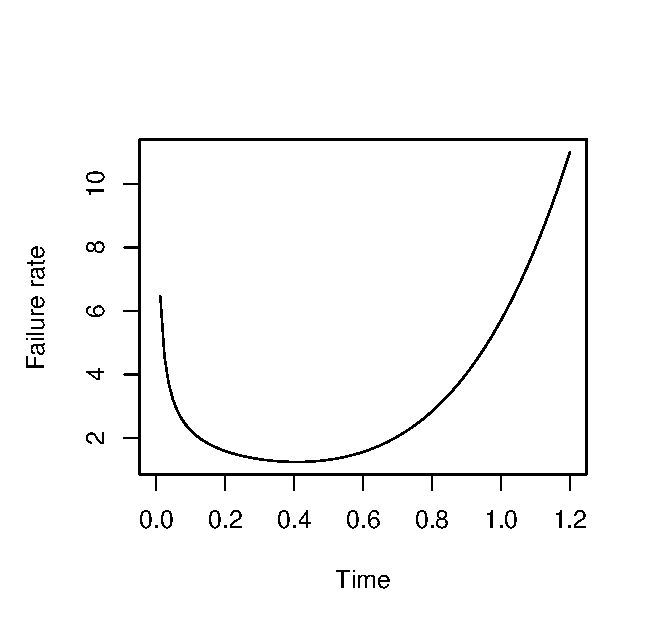
\includegraphics[height=9cm]{Fig1_motivatinghazard}%.eps}
\caption{Bathtub shaped failure rate.}\label{Fig:simulatedhazard}
\end{center}
\end{figure}

The results of the TTT-SiZer analysis are shown in Figure \ref{Fig:simulatedSizer}. The top-left panel shows the empirical TTT-plot for these data. The plot suggests a change of sign in convexity properties of the curve thus revealing the characteristics of the underlying  bathtub shaped failure rate. This is confirmed by the color maps which represent inferences about the TTT-curve as well as its first and second derivatives. The top-right panel presents the corresponding SiZer-0 map. In this case, it can be seen a change of color in the sense white to black indicating that the TTT-transform crosses the diagonal of the unit square from below, which is in accordance with a bathtub shaped failure rate while at the same time allows to arguing against the NBUE. The bottom-left panel presents the SiZer-1 map indicating a positive sign of the first derivative, as expected since the TTT-curve is defined as a cumulative integral function. Finally, the bottom-right panel shows the SiZer-2 map which tells us about the second derivative. This graph picks up the true features of the underlying hazard model. 
The plot shows that the hazard rate decreases significantly at the beginning (white color up to about the point 0.5). There is then a zero-crossing  signaled by the dark gray color  (between points 0.5 and 0.7), indicating that the hazard rate is constant. The hazard rate then increases to the point 0.95, as the black color indicates. This reveals a minimum of the hazard rate around 0.5.
  

\begin{figure}[htb]
\begin{center}
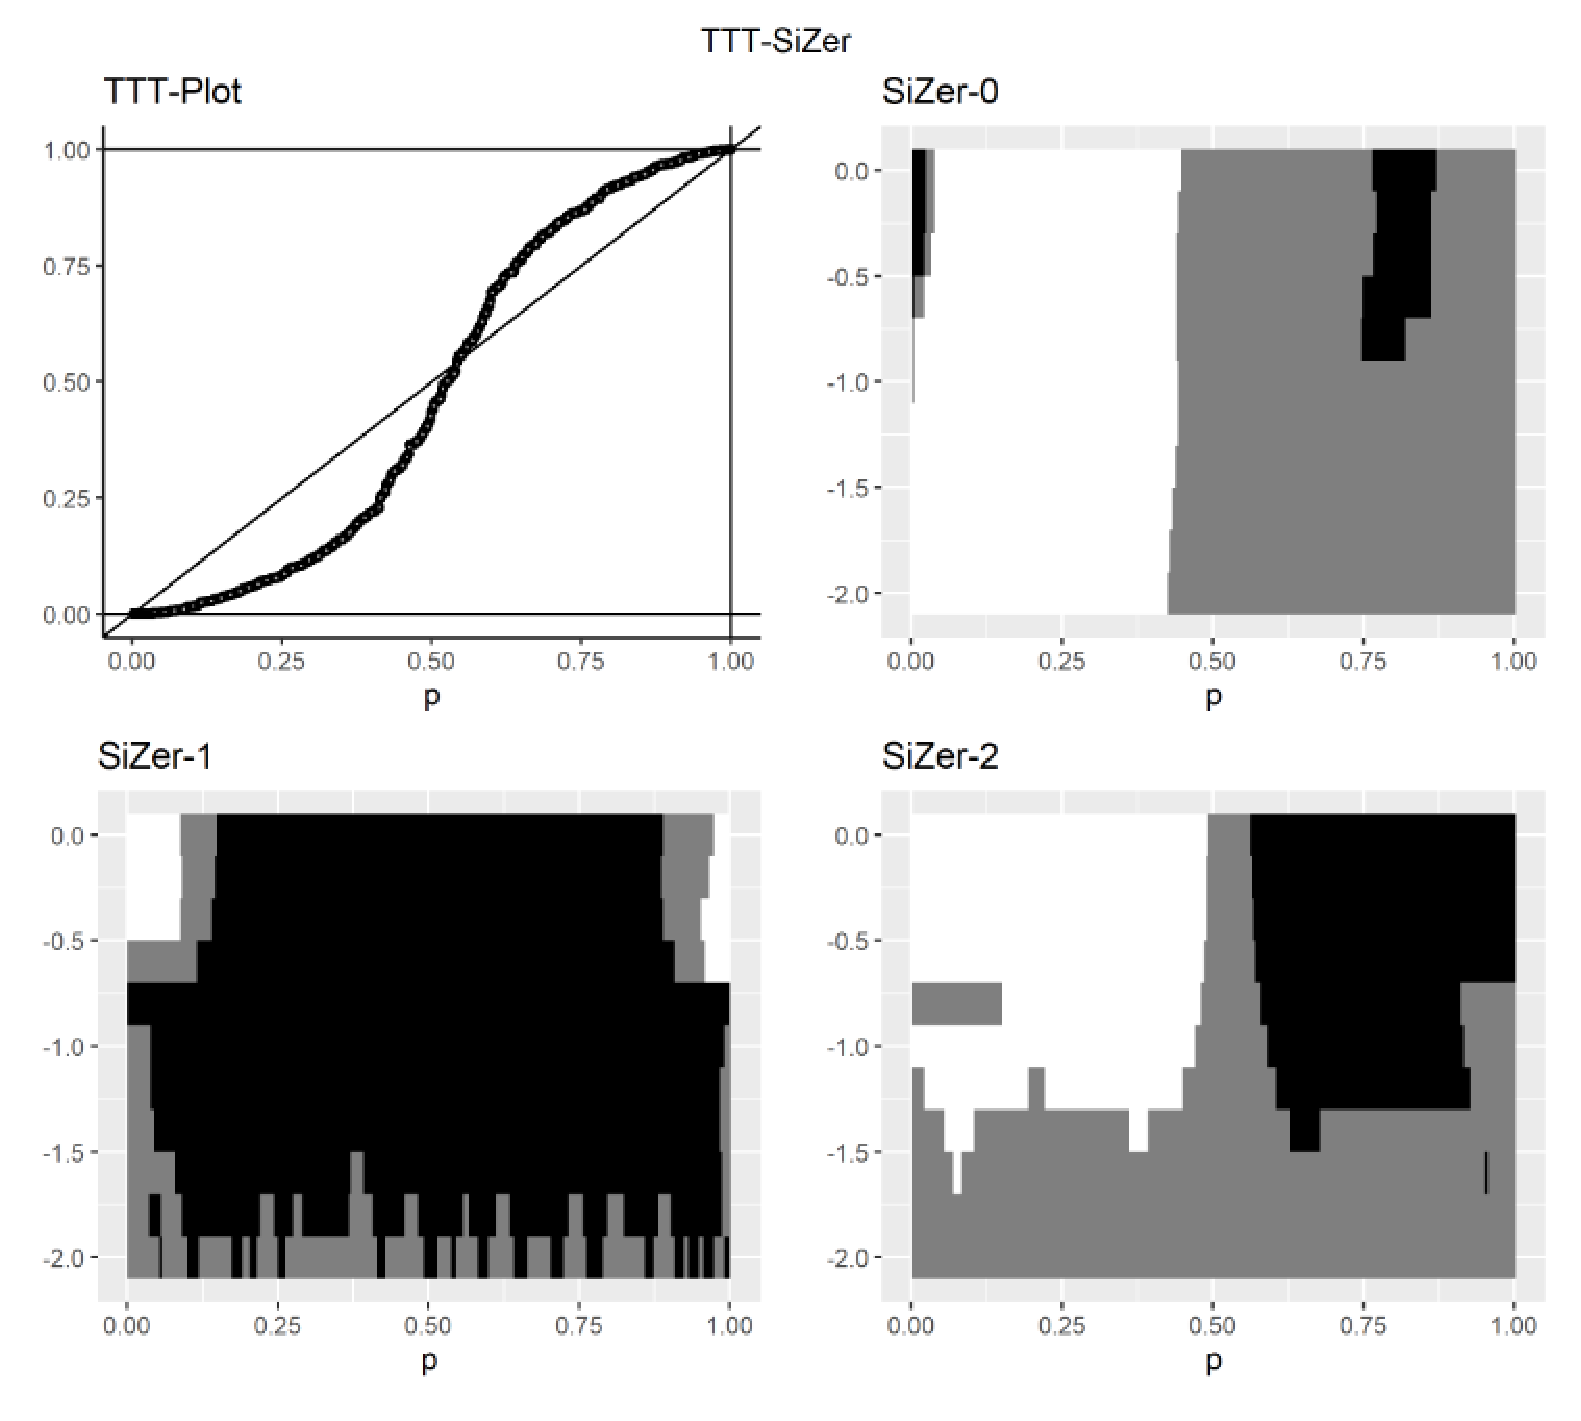
\includegraphics[height=9cm]{Fig2_motivatingSiZerCubic_log10}%.EPS}
\caption{TTT-Sizer for a dataset from an additive Weibull model.}\label{Fig:simulatedSizer}
\end{center}
\end{figure}

It is worth to mention at this point that, although  the same range of bandwidths is used for the three curves, it might not be the most appropriate. The second derivative implies the most complex estimation problem. More information is needed, meaning that bigger bandwidths are required. Smaller bandwidths increase variability. The resulting estimators are less efficient leading to wider confidence intervals. The wide dark gray area at the bottom of the plot in SiZer-2 shows this point.


%%%%%%%%%%%%%%%%%%%%%%%%%%%%%%%
\subsection{Some important issues in the SiZer methodology}
\begin{enumerate}
\item {\it Effective sample size} \\
\noindent The  concept of effective sample size (ESS) is considered as defined by \cite{CM99}. In this paper, an estimated slope is classified to be not enough data if its ESS is less than or equal to 5, 
$$
ESS(p_0,h) = \frac{\sum_{i=1}^n K_h(p_i-p_0)}{K_h(0)}.
$$

\item {\it Quantile functions} \\
\noindent Candidates for calculation of the quantile $q$ include:
\begin{itemize}
	\item Pointwise Gaussian quantiles: $q_1(h) = q_1 = \Phi^{-1}[1-\alpha/2]$, with $\Phi$ the standard normal distribution function. 
	\item Approximate simultaneous over $p$ Gaussian quantiles: based on ``number of independent blocks'' \cite{HM2006}, defined as
	$$
	q_2(h) = \Phi^{-1} \left[\left(1- \frac{\alpha}{2}\right)^{1/\left\{\theta(\Delta)d\right\}}\right],
	$$
	where
	$$
	\theta(\Delta) =2 \Phi \left\{ \frac{\Delta \sqrt{3 \log(d)}}{2h}\right\}-1,
	$$
	with $d$ the number of pixels in a row in the SiZer Map, $\Delta$ is the distance between two successive neighbouring locations $p_0$. In \cite{HM2006} the quantity $\theta(\Delta)$ is defined as the clustering index that measures the level of dependency between pixels. 
\end{itemize}
\end{enumerate}
%%%%%%%%%%
\subsection{Examples: Two real cases in Reliability}
In this section, the proposed graphic tool is applied to two real datasets. The first dataset (Example 1) represents interoccurrence
times of fatal accidents to British-registered passenger aircraft, 1946-1963, measured in number of days and listed in the order of their occurrence in time. The second dataset (Example 2) represents failure and running times (1000 cycles) of a sample of 30 units of a larger electrical system. The data have been taken from Appendix B of \cite{CMO2019}, where new consistent and scale-free goodness-of-fit tests for the Exponential distribution are presented. After an exhaustive analysis of the two real cases, the
authors conclude Exponential distribution is acceptable for the first case while not for the second one. Moreover, they point out that the proposed tests agree with the decisions suggested by different exponentiality tests with proven good power performance. However, they note that, at the 5\% level of significance, few of them fail to reject the null hypothesis for the second dataset.
In Figure \ref{Fig:2reliab_data} only partial information  provided by the SiZer analysis is reported, specifically the results based on inferences about the second derivative. On the top panel,  Example 1 is analyzed. The TTT-plot is displayed on the left side and the SiZer-2 map on the right. According to the arguments given in the former section, it can be concluded that the Exponential distribution fits well the data in this case. 
As for Example 2, a very different graph is produced so the Exponential distribution is clearly not admissible for the second case.

\begin{figure}[htb]
\begin{center}
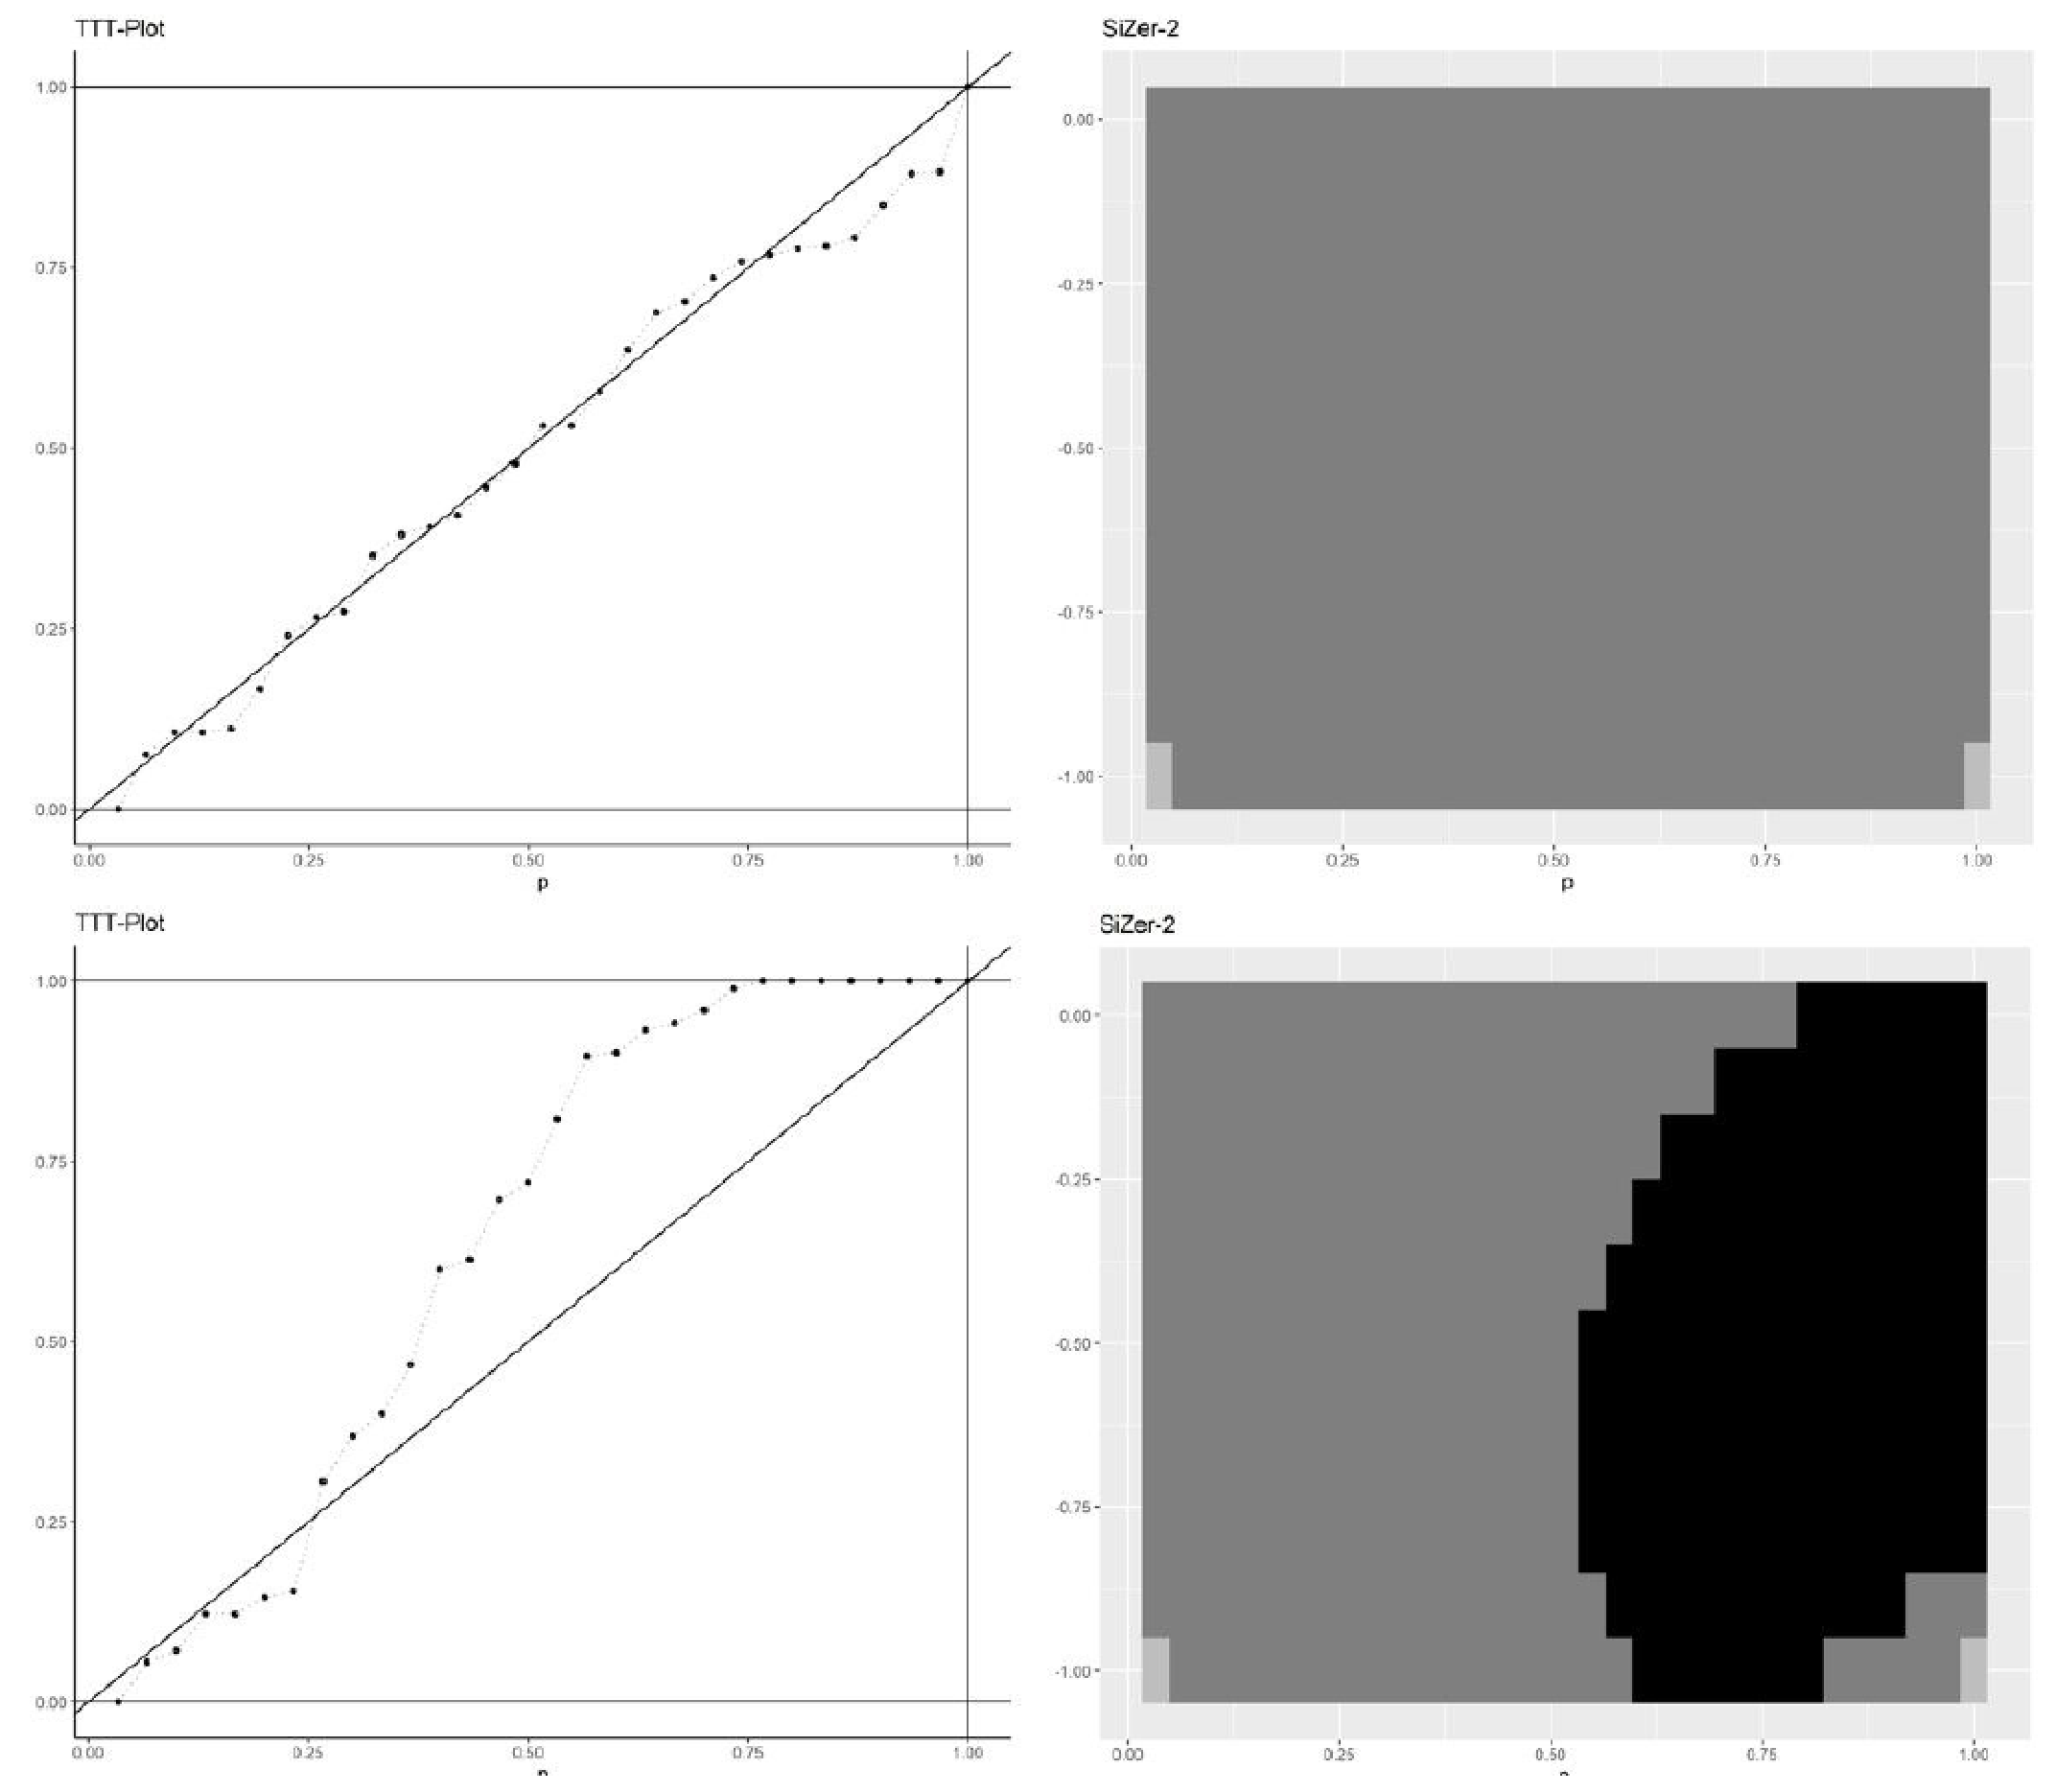
\includegraphics[height=9cm]{Fig3_twosamplestogether}
\caption{TTT-Sizer analysis of two real cases in Reliability.}\label{Fig:2reliab_data}
\end{center}
\end{figure}



%%%%%%%
\subsection{Hypothesis testing based on TTT-SiZer}

In this section, a graphical test based on TTT-SiZer is derived to explore aging  trends underlying in a given lifetime dataset. The null hypothesis ($H_0$) is ``No aging'', that is, the underlying lifetime is assumed to be exponentially distributed. Different alternative hypotheses ($H_1$) are faced according to the particular aging trend one is interested in. The kind of $H_1$ also determines the way the condition of ``No aging'' in $H_0$ is expressed. More specifically, a classic statistical testing problem can be settled  as follows:

 \noindent Let $X$ be a random lifetime,  one is interested in testing the null hypothesis 
\[
{\rm H_0 :} \ X \ {\rm follows \ Exp}(\lambda) \ {\rm distribution,\ for \ some \ } \lambda >0,
\]
against general alternatives based on a sample $X_1, X_2,\ldots, X_n$ of independent copies of $X$.

In order to solve the problem using the graphical test, the hypothesis is written in terms of the TTT-transform. In this sense, mainly the two following problems are considered: 
%%%%%%
\begin{enumerate}

\item ``No aging'' $against$ NBUE:
\begin{eqnarray} \label{test_nbue}
\nonumber &&{\rm H_0 :} \ \varphi_X(p)= p, {\rm for \ all \ } p \in (0,1); \\
&&{\rm H_1 :} \ \varphi_X(p) >  p, {\rm for \ some \ }  p \in (0,1).
\end{eqnarray}


\item ``No aging'' $against$ IFR:
\begin{eqnarray} \label{test_ifr}
\nonumber &&{\rm H_0 :} \ \varphi_X''(p)= 0, {\rm for \ all \ } p \in (0,1); \\
&&{\rm H_1 :} \ \varphi_X''(p) < 0, {\rm for \ some \ }  p \in (0,1).
\end{eqnarray}

\end{enumerate}



The proposed graphic tool is composed of  four plots: the TTT-plot and the three SiZer maps which are described below.

\begin{itemize}
\item SiZer-0:
\noindent The first map is based on the sign of the following transformation of the  TTT curve: $g_0(p)=\varphi(p) - p$.
Then,  the corresponding $(1-\alpha)100\%$ confidence interval for $g_0(p)$ is considered, that is 

\[
\left[\widehat{\varphi}_h(p)-q_{1-\frac{\alpha}{2}}\sqrt{\widehat{V}\left(\widehat{\varphi}_h(p)\right)}-p, \ \widehat{\varphi}_h(p)+q_{1-\frac{\alpha}{2}}\sqrt{\widehat{V}\left(\widehat{\varphi}_h(p)\right) }- p \right],
\]
\noindent for $0\leq p \leq 1$.


\item SiZer-1:
\noindent The second map examines the sign of the first derivative, then define $g_1(p)=\varphi'(p)$. This map is built just for checking purposes. Since the TTT-transform is defined as the integral of a positive continuous function, it should be an increasing function, and so it should be displayed in the SiZer-1 map. %The color code for this case is:...

\item SiZer-2:
\noindent In this case,  the sign of the second derivative of the TTT-transform is examined. Then  confidence intervals for $g_2(p)=\varphi''(p)$ are computed. For $0\leq p \leq 1$,
\begin{equation}\label{ci_d2phi}
\left[\widehat{\varphi}''_h(p)-q_{1-\frac{\alpha}{2}}\sqrt{\widehat{V}\left(\widehat{\varphi}''_h(p)\right)}, \ \widehat{\varphi}''_h(p)+q_{1-\frac{\alpha}{2}}\sqrt{\widehat{V}\left(\widehat{\varphi}''_h(p)\right)}\right].
\end{equation}

\end{itemize}
In all cases, $q$ is a proper quantile. The corresponding function $g_k(p)$, for $k =0,1,2$ is significantly positive (negative) when both confidence limits are above (below) 0, and it is not significant when 0 belongs to the confidence interval.

The general procedure consists of rewriting the hypotheses in SiZer language. To explain it, let us focus on \eqref{test_ifr}. The null hypothesis is equivalent to asserts that the  SiZer-$2$ map underlying to the true distribution is completely dark gray. This one is called the $true$ SiZer-2 map. The decision is to reject the null hypothesis in the case that the $empirical$ SiZer-2, which is the one based on the data,  displays a percentage of non-dark gray pixels above a pre-specified level.

This level is usually referred to as the type I error probability and it is denoted as $\alpha$. This value is commonly taken as $\alpha=0.05$. 

The steps of our proposal are summarized in the following algorithms. 

\subsection*{Algorithm 2. Testing exponentiality $against$ hazard-trend changes} 
Define the $true$ TTT-SiZer map according to an Exponential distribution. Under this null hypothesis, SiZer-2 is completely dark gray. 
\begin{enumerate}
\item[Step 1.] Compute the sample mean $\bar{X}$ and define $\bar{X}_i=X_i/\bar{X}$, for $ i=1,2,\ldots,n$.

\item[Step 2.] Construct the $empirical$ SiZer-$2$ map as explained in Section \ref{sizer1} based on  $\{\bar{\bf X}_i; i=1, 2,\ldots, n \}$.
\item[Step 3.] Compare pixel by pixel the $empirical$ SiZer-$2$ map with the corresponding $true$ SiZer-$2$ map and count the total number of pixels where the color in the generated $empirical$ map is not the same as in the $true$ map. Define the test statistic $T_2$, as the percentage of non-dark gray pixels in the empirical map, the reported value is $T_2^0$.

\item[Step 4.] Use bootstrap methods to approximate the distribution of statistic $T_2$ under $H_0$: Draw $M$ samples of size $n$ from the $Exp(1)$ distribution. Construct the corresponding Sizer-$2$ maps and count for each the number of non-dark gray pixels. A bootstrap sample of $T_2$, labelled $T^{*}_2$, is obtained.

\item[Step 5.] Define the $p$-value as $p_{2,boot}=(1/M)\sum_{m=1}^M I\left\{T^{*,m}_2 > T_2^0\right\}$, with $I\{\cdot\}$ an indicator function.
\end{enumerate}
Reject the null hypothesis at a significance level of $\alpha \in [0,1]$ when $p_{2,boot} < \alpha$. 



%%%%%%%%%%%%%%%%%%%%%%%%%%%%%%%%%%%%%  EXAMPLES

\subsection*{Example 3. Aarset dataset, \cite{A1987}}
For a demonstration of the above  testing method, let us consider the dataset consisting of $n=50$ failure times of electrical devices, available in \cite{A1987}. The results provided by classical tests are given in Table \ref{exp.test.aarset}.
As suggested by the TTT-plot, the interest, in this case, is to test exponentiality against BFR alternatives. The results of the TTT-SiZer method have been implemented for the local-cubic estimator and are presented in Figure \ref{Fig:aarset}. 
\begin{figure}[htb]
\begin{center}
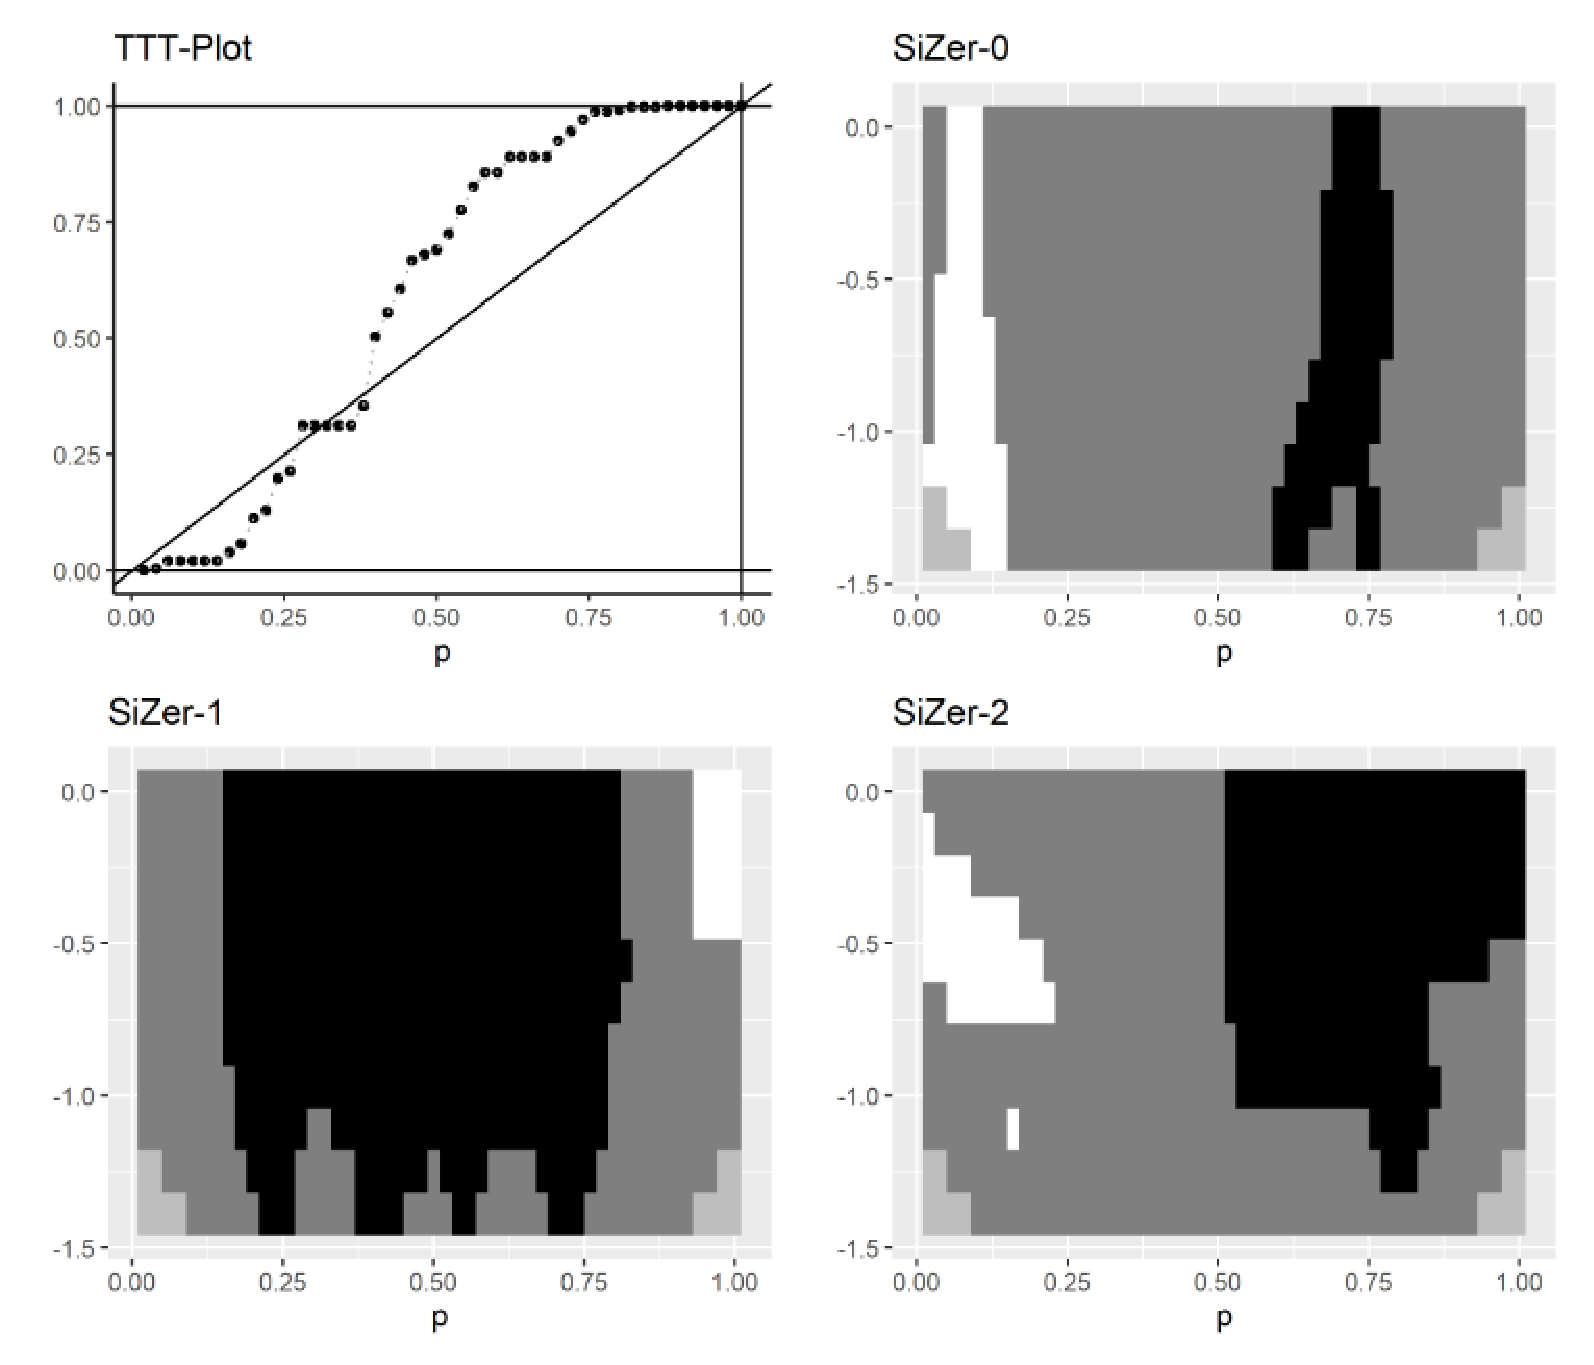
\includegraphics[height= 9cm]{Fig4_aarsetCubicPuntual_log10}%.EPS}
\caption{TTT-Sizer for Example 3: Electric devices failure times.}\label{Fig:aarset}
\end{center}
\end{figure}

Moreover, Algorithm 2 has been implemented for this data case. A total of $M=1000$ samples of size $n=50$ according to $H_0$ have been simulated. The reported p-value $p_{2,boot}=0.044$ leads to the decision of rejecting Exponentiality, as also is suggested by the majority of testing procedures reported in Table \ref{exp.test.aarset}. Looking at the whole group of plots in Figure \ref{Fig:aarset} one can get more information than the only provided by the p-value. As already mentioned, the TTT-plot suggests the BFR condition for the underlying lifetime. This idea is confirmed by looking at both SiZer-0. This graph displays a change of sign from white to black for all bandwidths which means that the data are not in accordance with the NBUE condition. On the other hand, looking at the plot presented on SiZer-2, there is an evident change from white to black meaning a clear change of trend of the hazard rate from decreasing to increasing. So, the conclusion is that the data come from a BFR lifetime distribution. 
This dataset has been frequently used by many reliability researchers for illustration purposes. Recently, it is used in \cite{KBM2020} to examine the performance of a new procedure aimed to estimate the point at which the $\mu_t$ function changes trend. The estimated change-point turns out to be 60 and 95\% confidence interval is given by (18, 79). Figure \ref{Fig:aarset} gives an overall picture of the inference about the TTT curve at a 95\% of confidence. It can be seen that between the quantiles 0.25 and 0.5 of the distribution, that is, the time scale interval (13.50, 64.6), the estimated confidence intervals are represented by dark gray pixels meaning that the zero is within the limits. The TTT curve presents a change of sign of convexity in this region. Our results are in accordance with \cite{KBM2020}.
%



\begin{table}
\centering
\caption{Example 3. Some Exponentiality tests implemented in package $exptest$ \cite{NPY15} of program R.}
\begin{tabular}{|l|c|c|}  \hline
{\bf Test  }\cite{Ascher90} & Test Statistic & $p$-{ value}  \\ \hline
Cox and Oakes        & $-3.388$ & 0.709 \\ \hline
Cramer-von Mises    & $ 0.519$ &  1 \\ \hline
Deshpande            & $0.708$   &  0.528  \\ \hline 
Gini-statistic      & $ 0.411$   &  {\bf 0.031} \\ \hline  
Gnedenko $F$-test  &  $2.236$     & {\bf 0.005 } \\ \hline 
Hollander- Proschan  &$0.209 $ & {\bf 0.007}   \\ \hline 
Kochar            &  $ 3.509$ & {\bf 0.0004 } \\ \hline 
Kolmogorov-Smirnov & $0.191$ & {\bf 0.005}  \\ \hline 
Lorenz test        & $0.177 $& 0.870 \\ \hline 
Shapiro-Wilk   & $ 0.040$ & 0.996 \\ \hline  
\end{tabular}
\label{exp.test.aarset}
\end{table}

\subsection*{Algorithm 3. Testing exponentiality $against$ NBUE alternatives} 
Define the $true$ TTT-SiZer map according to an Exponential distribution. Under this null hypothesis, SiZer-0 is completely dark gray. 
\begin{enumerate}
\item[Step 1.] Compute the sample mean $\bar{X}$ and define $\bar{X}_i=X_i/\bar{X}$, for $ i=1,2,\ldots,n$.
\item[Step 2.] Construct the  $empirical$ SiZer-$0$ map as explained in Section \ref{sizer1} based on  $\{\bar{\bf X}_i; i=1, 2,\ldots, n \}$.
\item[Step 3.] Compare pixel by pixel the $empirical$ SiZer-$0$ map with the corresponding $true$ SiZer-$0$ map and count the total number of black pixels in the generated $empirical$ map, which means that the curve is strictly above the diagonal. Define the test statistic $T_0$, as the percentage of black pixels in the empirical map, the reported value is $T_0^0$.

\item[Step 4.] Use bootstrap methods to approximate the distribution of the statistic $T_0$ under $H_0$: Draw $M$ samples from the $Exp(1)$ distribution. Construct the corresponding Sizer-$0$ maps and count for each the number of black pixels, then a bootstrap sample of $T_0$, labelled $T^*_0$, is generated.

\item[Step 5.] Define the $p$-value as $p_{0,boot}=(1/M)\sum_{m=1}^M I\left\{T^{*,m}_0 > T_0^0\right\}$.
\end{enumerate}
Reject the null hypothesis at a significance level $\alpha \in [0,1]$ when $p_{0,boot} < \alpha$. 
 

To illustrate this method, consider the following example. 
\subsection*{Example 4. Failure times of rear brakes, \cite{CMO2019}}
This dataset represents failure times for right rear brakes on D9G-66A Caterpillar tractors \cite{CMO2019}. The null hypothesis of Exponential distribution is clearly rejected by the classical test, and the TTT-plot also points to this decision. The graphical test has been carried out using the local-cubic estimator and paying attention to the alternative hypothesis $H_1$: ``NBUE but not Exponential distribution''. In this case, the plot presented in SiZer-0 shows that data are in accordance with $H_1$. Moreover, Algorithm 3 has provided a value for the statistics $T_0^0=0.663$ with a value $p_{0,boot}=0.000$, which suggests clear evidence in that sense. 

\begin{figure}[htb]
\begin{center}
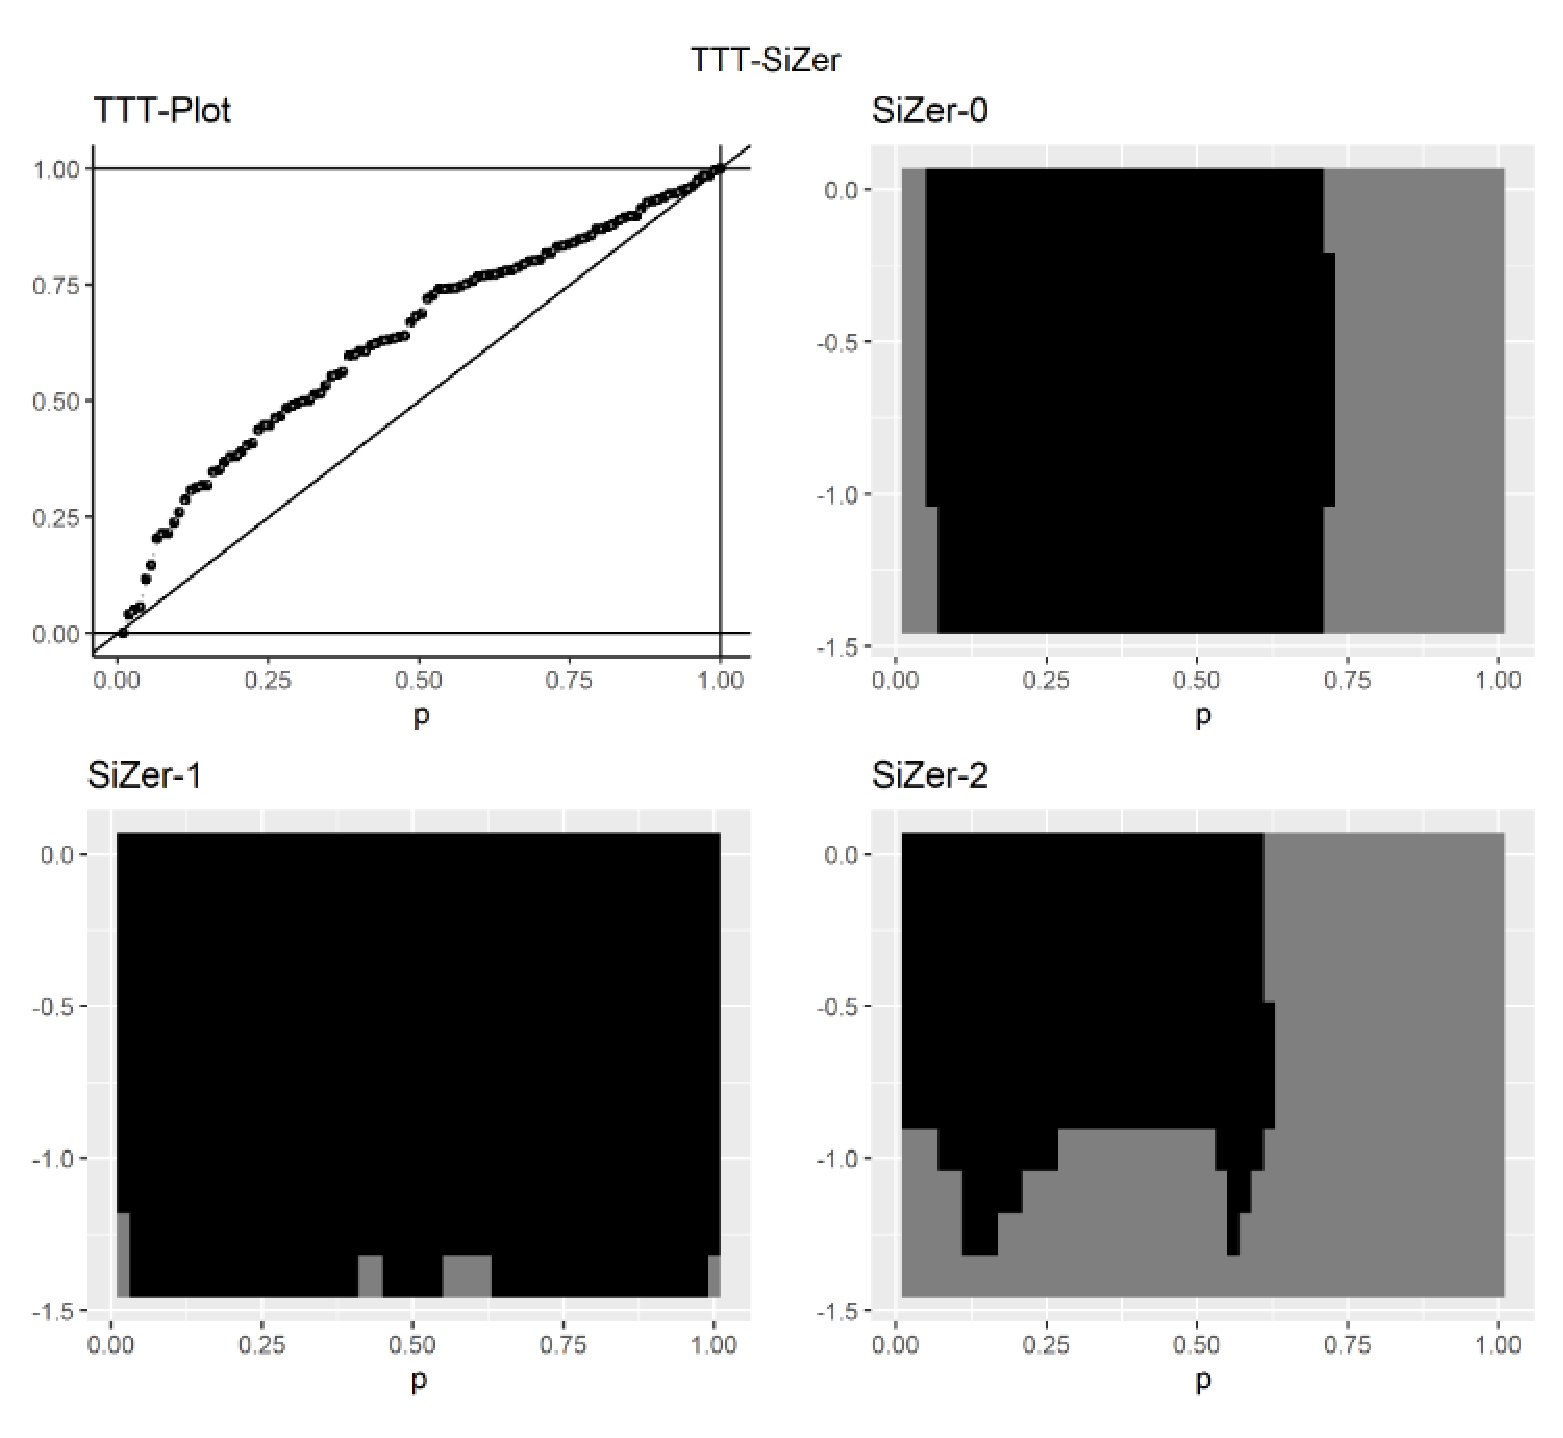
\includegraphics[height= 9cm]{Fig5_brakes_log10}%.EPS}
\caption{TTT-Sizer for Example 4: Failure times dataset of a brake-system.}\label{Fig:brakes}
\end{center}
\end{figure}
%

%\bigskip
%%%%%%%%%%%%
\section{Simulations}\label{sec:sim}
In this section, the performance of the graphical test is evaluated. The type I error of the test and the empirical power under different alternatives are calculated.


\subsection{Type I error}
The type I error occurs when the graphical test rejects the true model under the null hypothesis. To evaluate the type I error of the graphical TTT-test, samples of size $n$ = 50, 100, 500, and 1000, from an Exponential distribution with mean 1 are simulated.

The TTT-transform and its second derivative are estimated using the local polynomial estimators defined in Section \ref{locpol}, with the gaussian kernel.  
The algorithm consists of simulating a sample of size $n$ from the true model, then the local-polynomial estimate is calculated and the TTT-SiZer method is applied to compare the SiZer-$j$ map (for $j=0,2$) with the corresponding true one.

The probability of committing this error is calculated following \cite{RMP07}. The null hypothesis is $H_0$: \textit{No aging} and the  alternative is  $H_1$: \textit{``Aging trend''}. Two different tests are performed. On the one hand, when the alternative is ``NBUE but not Exponential'', aging trends are sought by inspecting the TTT-curve in the SiZer-0 map. 
Stronger conditions such as ``IFR but not Exponential'' can be elucidated by studying the SiZer-2 map. In any of the two cases, under the null hypothesis, the corresponding generated map should have only dark gray pixels.  Let us focus on the SiZer-2 map case to explain the procedure to study the type I error.\\
 
As remarked above, under the null hypothesis that the TTT-curve is the diagonal of the unit square, the SiZer-2 map  should have only dark gray pixels. This map is considered as the true one. The experiment is repeated $M=1000$ times.  For all the $M$ simulated samples, the corresponding SiZer-2 maps are constructed  and compared with the true map, pixel by pixel. For each sample,  the total number of pixels where the color in the generated map is not the same as in the true map is recorded. The proportion of type I errors for each sample is this count divided by the total number of pixels in the map.  $M$ proportions of type I errors (one for each simulated sample) are obtained for each sample size. Table \ref{Tab:errorI} presents summary statistics from the experiment and reports results for the two tests, which are for alternative NBUE and IFR, respectively. 


\begin{table}[htb]
\centering
\caption{Summary statistics of the type I errors calculated from $M=1000$ simulated samples, for the null hypothesis of $ H_0$: No aging. Columns 2-4 report the mean, the median and the quantile of order 0.75 for the proportions of type I error for the test with alternative $H_1$: NBUE.  Columns 5-7 report the mean, the median and the quantile of order 0.75 for the proportions of type I error for the test with alternative $H_1$: IFR.}
{\begin{tabular}{r|ccc|ccc}\hline
               & \multicolumn{3}{|c|}{$SiZer-0$}& \multicolumn{3}{c}{$SiZer-2$} \\ \hline
   Sample size & Mean &   Median & $P_{75}$ &  Mean &   Median & $P_{75}$  \\ \hline
       50      &  0.011 &0.000 &0.000 &   0.036 & 0.000 & 0.017  \\
      100      &  0.014 &0.000 &0.000 &   0.033 & 0.001 & 0.026  \\
     500       &  0.012 &0.000 &0.004 &   0.028 & 0.008 & 0.027 \\
     1000      &  0.012 &0.000 &0.003 &   0.035 & 0.013 & 0.034 \\ \hline
\end{tabular}}
\label{Tab:errorI}
\end{table}
 Table \ref{Tab:errorI}  shows that the mean of the proportions of type  I error is under 5\% for all sample sizes, as well as the median.

\subsection{Empirical power}

In hypothesis testing the power is defined as the probability of rejecting the null hypothesis when it is false. The probability of accepting the null hypothesis when false is called type II error. To evaluate the power of the graphical TTT-test, three  different aging models and sample sizes $n = 50, 100, 500$, and $1000$ are considered, as in the previous section.  In particular:
\begin{itemize}
\item IFR model: $X_1$ with Gamma distribution with shape parameter $sh=5$ and mean $\mu=1$;
\item BFR model: $X_2= \min\{W_1, W_2, W_3\}$, where $W_j$ has Weibull distribution with scale $sc=2.5$, and respectively, shape parameters given by $sh_1=3$, $sh_2=2$, and, $sh_3=0.5$;
\item UFR model: $X_3$ with log-Normal distribution with parameters $E[ \log (X_3)]=-0.5$, and $Var(\log(X_3))=1$.
\end{itemize}
In all cases, the parameters have been chosen to have mean around 1 and avoid scale adjustments of the TTT transform. A picture of the corresponding hazards is given in Figure \ref{models}.

The TTT-transform and its first and second derivatives are estimated using the local polynomial estimators defined in Section \ref{locpol}, with the gaussian kernel. The TTT-SiZer method is applied to visualize the inference about the three curves considering for each case the corresponding two-dimensional space with $np \times nh$ pixels, respectively.  

\begin{figure}[h]\centering
        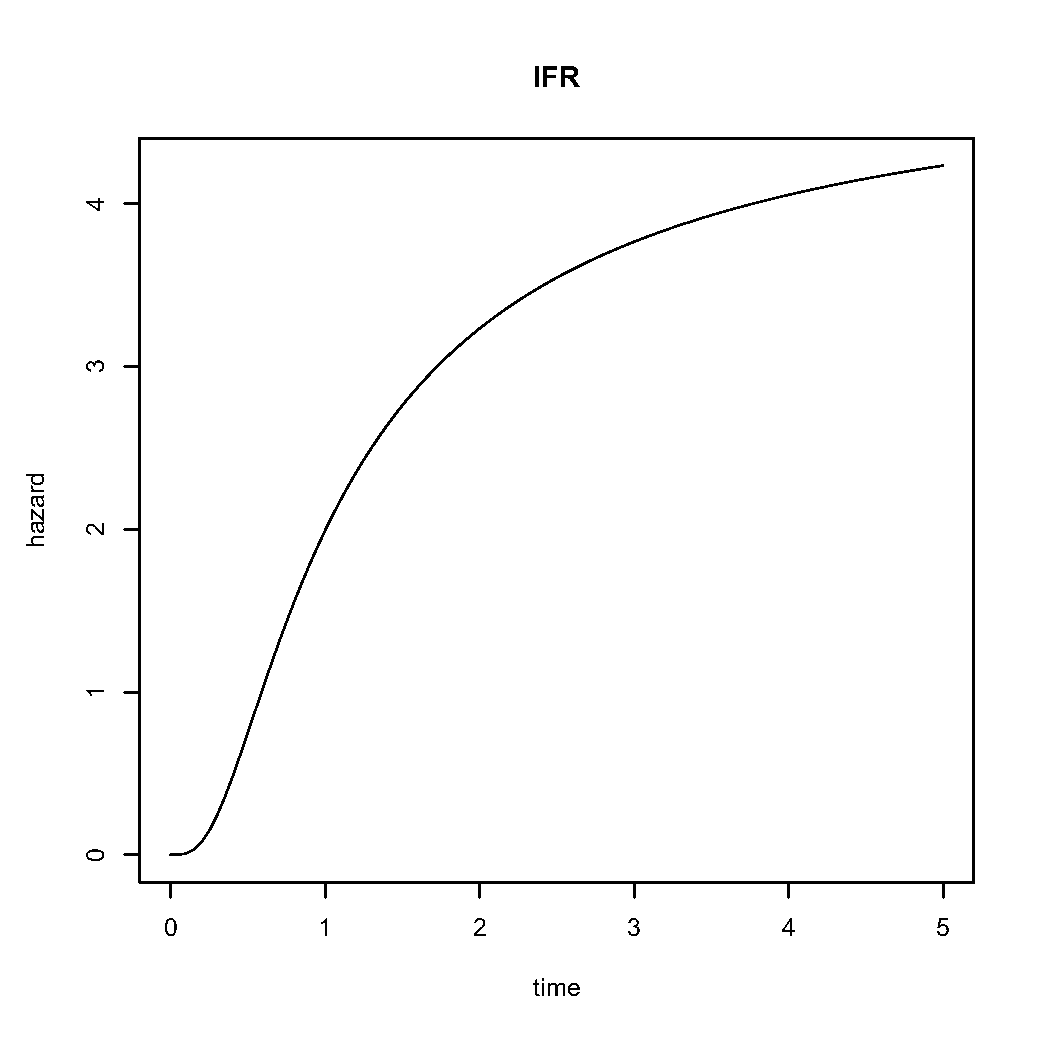
\includegraphics[height=4.5cm]{Fig6_1_IFRmodel}%.eps}
				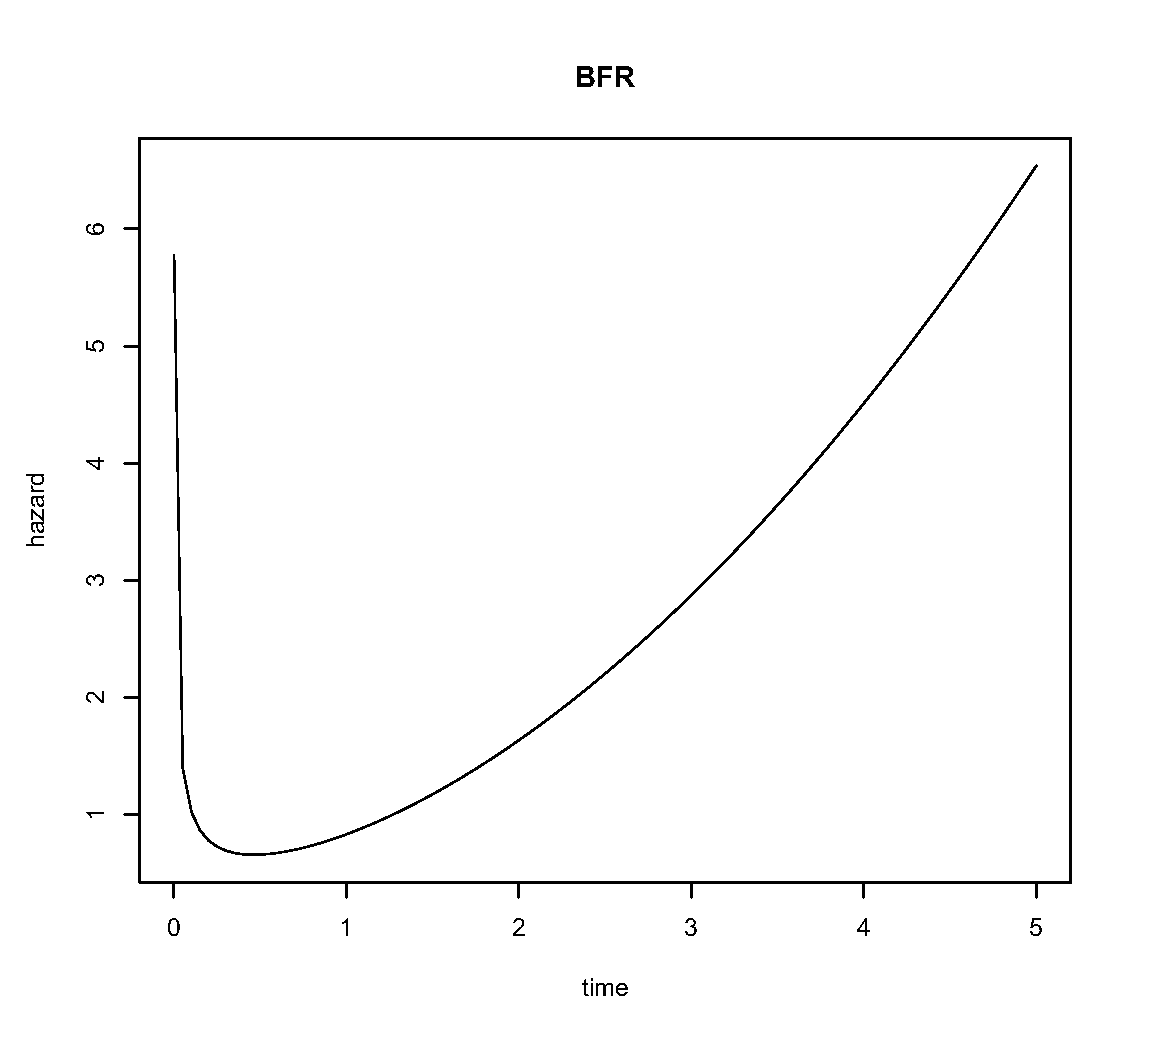
\includegraphics[height=4.5cm]{Fig6_2_BFRmodel}%.eps}
				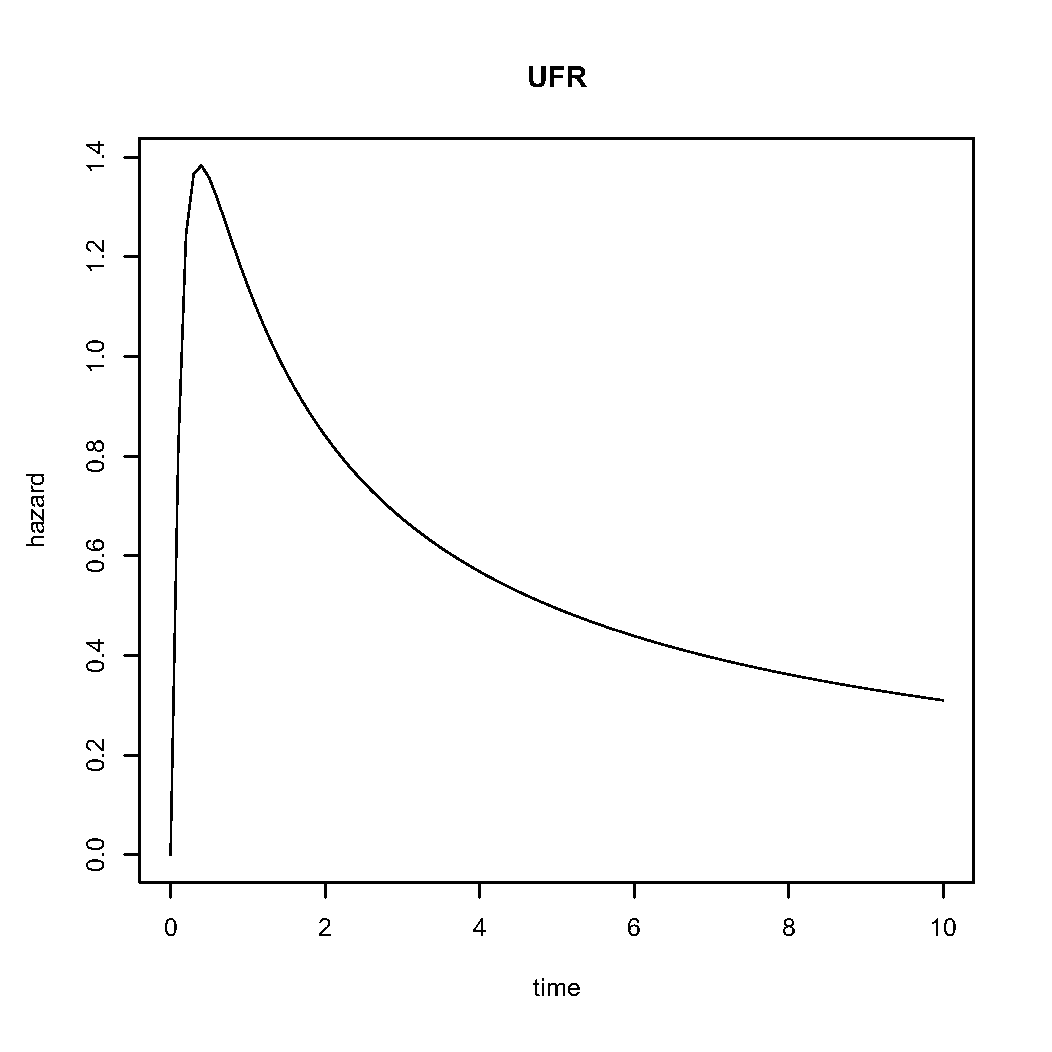
\includegraphics[height=4.5cm]{Fig6_3_UFRmodel}%.eps}
\caption{{Hazard functions for the three aging models considered}.} \label{models}
\end{figure}

The algorithm now consists of simulating a sample of size $n$ from the true model, then  the local-polynomial estimate is calculated and the TTT-SiZer method is applied to compare the corresponding set of maps with the true ones.
The type II error occurs when the graphical test accepts the null hypothesis under the alternative. Each model represents a different  aging trend in some way. Under the null  hypothesis, the SiZer-2 map  should have only dark gray pixels. This map is the true one. The experiment is repeated $M=1000$ times.  For each of the $M$ simulated samples,  the corresponding maps are constructed and compared with the true map, pixel by pixel. For each sample, the total number of pixels where the color in the generated map is  the same as in the true map is recorded. The proportion of type II errors for each sample is this count divided by the total number of pixels in the map. $M$ proportions of type II errors (one for each simulated sample) are obtained for each sample size. The empirical power is obtained as one minus this proportion. Table \ref{Tab:power} presents the results of the experiment.


\begin{table}[htb]
\centering
\caption{Summary of empirical power calculated from $M=1000$ simulated samples.}
{\begin{tabular}{llllllll} \hline
  $H_1$   & Sample size &   Mean & Min. & Median   & $P_{75}$ & $P_{95}$& Max.\\
\hline
IFR model &50        & 0.746& 0.035 & 0.771 & 0.805  & 0.861 & 0.908\\
          &100       & 0.651& 0.444 & 0.654 & 0.679  & 0.711 & 0.747\\
          &500       & 0.517& 0.461 & 0.518 & 0.529  & 0.544 & 0.560\\
          &1000      & 0.557& 0.521 & 0.558 & 0.567  & 0.580 & 0.589\\ \hline
BFR model &50        & 0.184& 0.000 & 0.143 & 0.234  & 0.610 & 0.762\\
          &100       & 0.243& 0.000 & 0.221 & 0.285  & 0.528 & 0.647\\
          &500       & 0.390& 0.240 & 0.398 & 0.454  & 0.490 & 0.525\\
          &1000      &0.499 & 0.360  & 0.516 & 0.533  & 0.552 & 0.568\\ \hline
UFR model &50        &0.050 & 0.000 & 0.008 & 0.043  & 0.340 & 0.670\\
          &100       &0.093 & 0.000  & 0.089 & 0.098  & 0.456 & 0.600 \\
          &500       &0.305 & 0.006  & 0.350 & 0.403  & 0.445 & 0.495\\
          &1000      &0.430 & 0.157  & 0.448 & 0.471  & 0.490 & 0.506\\ \hline

\end{tabular}}
\label{Tab:power}
\end{table}

Note that for sample sizes $n=500, 1000$ the maps have been built taking in total $401 \times 11$ pixels, whereas for $n=100$, $51 \times 11$ pixels, and for $n=50$, $21 \times 11$ pixels are considered in the maps, which means that the results are not fully comparable. Table \ref{Tab:power} shows the good performance of our test given that the results presented in the table imply a percentage of rejection is reasonable to high for almost all models and sample sizes. Especially when the alternative hypothesis is monotone. Only for the UFR case and small sample sizes, a small percentage of pixels allowing  to detect the alternative hypothesis in the data are obtained. For the rest of the models and sample sizes, the graphical test displays wide areas in the corresponding plots properly recognizing the alternative hypothesis.


\section{Concluding remarks}


Nonparametric classification of lifetimes enables one to understand aging behaviors without a compromise with a definite parametric form of the underlying distribution. This makes the model less restrictive and much more robust (\cite{KM2019}) and is one important reason for the wide scope of applicability of the approach in this paper. 
Having an accurate idea of ​​an equipment or system aging profile can be of great help for engineers to design efficient age replacement maintenance policies. In modern industry, maintenance policies are designed to prevent high costs and, in some circumstances, even personal and environmental hazards caused by the occurrence of failures during the operation of complex systems and equipment, and so age replacement policy has an important role as a strategy for preventive maintenance.
 It is known that many real systems do not exhibit a monotone age pattern. Detecting and locating  different aging-trends along the life of a device or system, in the absence of precise knowledge about the distribution, is an important issue in reliability applications. 

In this line, this paper has aimed to present a new procedure to explore lifetime data for discovering aging trends and changes of tendency in the underlying life distribution which may have important implications in the context of cost optimization in age-maintenance policies.


A new estimator of the TTT-transform is obtained based on nonparametric statistics, more specifically, based on kernel smoothing techniques. Although nonparametric smoothing techniques are very popular in related areas such as survival analysis they are not very usual in reliability engineering where parametric methods have been traditionally preferred by the practitioners for solving inference problems. 
Although, the theoretical TTT transform is usually approximated from available data by means of the TTT-plot, which is a discontinuous curve while the theoretical curve is an absolutely continuous function. So, the empirical curve may be viewed as a poor approximation of the true curve, among other reasons, because it is a step function and the derivative either equals zero or is not defined, which makes it difficult to evaluate shape characteristics. Kernel smoothing avoids discontinuities in the empirical function.
Local-polynomial estimators have been constructed for the TTT-curve and its first and second derivatives. To obtain the properties of the estimators the moments of the order statistics have to be estimated and bootstrap methods have been considered for this purpose.

%%%%%%%%%%%%%%%%%%%%%%%%%%%%%%%%%%%%%%%%%%%%%%%%%%%%%%%%%%%%%%%%%%%%%%%%%%%%%%%%%%%%%%%%%%%

 
A graphic tool has been developed to test exponentiality against alternatives that represent non-constant trends in aging. This issue is not new in the reliability literature.  Klefsjo  in \cite{Klefsjo83a}, where, the author, guided by the properties of the TTT-transform, provides a series of hypothesis tests to contrast the exponentiality against a wide range of aging alternatives.
  Also remarkable is the work by \cite{A1987} where a test statistic based on the TTT plot, for testing if a random sample is generated from a life distribution with constant versus bathtub shaped hazard rate.
 The testing method proposed here is a graphical test able to recognize aging trends from data. The main advantage, compared to existing tests, is that it allows identifying specific areas where discrepancies from non-aging are detected. In contrast, standard testing methods summarize the sampling information in the single p-value to decide on the adequacy of the model specified in the null hypothesis.

  This graphical test is developed through scale and space inference about the Total-Time-on-Test transform which is implemented by adapting the SiZer methodology to our context. Punctual as well as simultaneous confidence intervals have been constructed around each curve and for different levels of smoothing. The graphical representation allows one to detect and confirm monotone aging trends and/or changes of tendency.
Simulations and the comparison with other non-graphical tests show that the graphical test helps localize discrepancies of empirical data concerning a given hypothesized aging property. The extensive simulation study carried out as well as the real cases discussed along the manuscript demonstrate that this proposal is interesting and has a high potential for reliability engineering in practice. 

A natural extension of the method is to consider more general scenarios where censoring and/or other filtering schemes are present in the sampling mechanism.



%\bigskip
%%%%%%%%%%%%%%%%%%%%%%%%%%%%%%%%%%%%%%%%%%%%%%%%%%%%%%%%%%%%%%%%%%%%%%%%%%%%%%%%%%%%%%%%%%%%%%%%%%%%%%%%%%%%%%%%%%%%%%%%%%%%%%%%%%
\section*{Acknowledgments} The authors are grateful for constructive comments from four anonymous Reviewers and the Associate Editor. This work has been partially supported by ERDF / Ministry of Science and Innovation - State Research Agency through grant number RTI2018-099723-B-I00. The authors thank Centro de Servicios de Inform\'atica y Redes de Comunicaciones (CSIRC), University of Granada, for providing the computing time. 


%
%%%%%%%%%%%%%%%%%%%%%%%%%%%%%                     APPENDIX

\appendix
%%%%%%%%%%%%%%%%%%%%%%%%%%         LOCAL- CUBIC

\section{The local-cubic aproach} \label{ap:cubic}
It is convenient to increase the complexity of the model when interested in exploring shape properties through the second derivative.
Thus it is proposed to carry out the local fit by using cubic polynomials. After solving the equations in \eqref{score} with $m=3$, taking  the empirical estimator given in \eqref{empi},  the estimators of $\varphi$ and its first and second derivatives can be written similar to Section \ref{quad} as follows.
%

%%%%%%%% TTT CURVE
\subsection{The TTT-curve }%{$\widetilde{\varphi}_h(p_0)=\widetilde{\theta}_0(p_0)$}

\noindent First, some notation is given. Let ${\bf A}$ be a square matrix of dimension $n \times n$. 

For each $i, j =1,2,\ldots, n$, denote $M_{i,j}$ corresponding $minor$, that is, the determinant of the sub-matrix obtained by deleting the $i$th row and the $j$th column of matrix ${\bf A}$. The corresponding $cofactor$ is given by  $\Delta_{ij}=(-1)^{i+j} M_{i,j}$. 

The Cramer's rule provides an appropriate solution of the system of linear equations and the determinants are computed by cofactor expansions. Then the solution is written as
\begin{equation}\label{phi.cub}
\widetilde{\varphi}_h(p_0)\left(p_i-p_0\right)= \widetilde{\theta}_0(p_0)=\sum_{i=1}^n \widetilde{K}_{0,h}\left(p_i-p_0\right) \widehat{\varphi}_{n,i},
\end{equation}
where the cubic kernel is expressed as
\begin{eqnarray*}
\widetilde{K}_{0,h}\left(p_i-p_0\right)&=& \\
&=&\frac{\Delta_{11}+\Delta_{21}\left(p_i-p_0 \right)+\Delta_{31}\left(p_i-p_0 \right)^2+\Delta_{41}\left(p_i-p_0 \right)^3}{a_0 \Delta_{11}+ a_1 \Delta_{21}+a_2 \Delta_{31}+a_3 \Delta_{41}} K_h\left(p_i-p_0\right),
\end{eqnarray*}
where the cofactors $\Delta_{ij}$, $i,j=1, 2, 3, 4$, are taken from matrix ${\bf A}$, that is,
\[
{\bf A} =\left(\begin{array}{cccc}
a_0 & a_1&a_2 &a_3 \\ 
a_{1} & a_2&a_3 &a_{4}\\
a_2 & a_3 &a_4 &a_5 \\ 
a_3 & a_4&a_5 &a_{6} 
\end{array}\right).
\]

\bigskip

%\subsection{The local-cubic estimator as an L-estimator}
The local-cubic estimator can be seen as an L-estimator likewise the second-order case (see Section \ref{stat_prop}) so the statistical properties of the estimator can be studied,  in particular, expressions for the moments are obtained next.

\begin{equation*}
\widetilde{\varphi}_h(p_0)= \sum_{i=1}^n \sum_{j=1}^i \widetilde{K}_{0,h}(p_i-p_0)\omega_{i,j}X_{(j)},
\end{equation*}
which is also an $L$-estimator, with $\omega_{i,j}$ as in \eqref{eq:omega}. Let us denote 
$$\widetilde{\bf K}_{0,h}(p_0)=\left(\widetilde{ K}_{0,h}(p_1-p_0), \widetilde{ K}_{0,h}(p_2-p_0),\ldots,\widetilde{ K}_{0,h}(p_n-p_0)\right)^{\intercal},$$
 so the variance of the estimator of the TTT-curve using the local-cubic approach is
\begin{equation}\label{V.phi0.cubic}
{\rm Var} \left(\widetilde{\varphi}_h(p_0)\right)= \widetilde{\bf K}_{0,h}(p_0)^{\intercal}\cdot {\bf W} \cdot {\boldsymbol{\Sigma}}\cdot  {\bf W}^{\intercal}\cdot \widetilde{\bf K}_{0,h}(p_0),
\end{equation}
for each $p_0 \in (0,1)$. Equally the variance for the first and second derivatives of the local-cubic estimate can be obtained.
 
%%%%First derivative:

\subsection{The first derivative} %{$\widetilde{\varphi'}_h(p_0)=\widetilde{\theta}_1(p_0)$}
\begin{equation}\label{dphi.cub}
\widetilde{\varphi}'_h(p_0)=\widetilde{\theta}_1(p_0)= \sum_{i=1}^n \widetilde{K}_{1,h}\left(p_i-p_0\right) \widehat{\varphi}_{n,i},
\end{equation}
where
\begin{eqnarray*}
\widetilde{K}_{1,h}\left(p_i-p_0\right)&=& \\
&=&\frac{\Delta_{12}+\Delta_{22}\left(p_i-p_0 \right)+\Delta_{32}\left(p_i-p_0 \right)^2+\Delta_{42}\left(p_i-p_0 \right)^3}{a_0 \Delta_{11}+ a_1 \Delta_{21}+a_2 \Delta_{31}+a_3 \Delta_{41}}  K_h\left(p_i-p_0\right). \qquad
\end{eqnarray*}


%%%% Second derivative:

\subsection{The second derivative}%{ $\widetilde{\varphi''}(p_0)=2\widetilde{\theta}_2(p_0)$}
Finally the second derivative, based on local-cubic approximation.
\begin{equation}\label{d2phi.cub}
\widetilde{\varphi}''_h(p_0)= 2 \widetilde{\theta}_2(p_0)= \sum_{i=1}^n \widetilde{K}_{2,h}\left(p_i-p_0\right) \widehat{\varphi}_{n,i},
\end{equation}
where 
\begin{eqnarray*}
\widetilde{K}_{2,h}\left(p_i-p_0\right)&=&\\
&=& \frac{\Delta_{13}+\Delta_{23}\left(p_i-p_0 \right)+\Delta_{33}\left(p_i-p_0 \right)^2+\Delta_{43}\left(p_i-p_0 \right)^3}{a_0 \Delta_{11}+ a_1 \Delta_{21}+a_2 \Delta_{31}+a_3 \Delta_{41}} K_h\left(p_i-p_0\right).
\end{eqnarray*}



%%%%%%%%%%%%%%%%%%%%%%%%%%%%%%%%%%%%%%%%%%%%%%%%%%%%%%%%%%%%%%%%%%%%%%%%%%%%%%%%%%%
\section{Bootstrap moments of the order statistics} \label{apx:moments}

Following \cite{HE2000}  the estimators above are considered as L-estimators  and  bootstrap techniques can be used to estimate the first two moments of the order statistics, that is, vector $\boldsymbol{\mu}$, given in \eqref{mean}, and the covariance matrix $\boldsymbol{\Sigma}$ given in \eqref{var}. 


Exact analytic expressions for these bootstrap mean and covariance matrix are obtained, as well as the corresponding estimators based on Monte Carlo resampling. 

\subsection{Exact analytic expressions}

Let $X_1,X_2,\ldots, X_n$ be a sample of independent random variables with a common absolutely continuous distribution $F$, and let  $X_{(1)} \leq X_{(2)}\leq \cdots X_{(n)}$ be the order statistics. 

First,  define $m$th non-centered moment of the $r$th order statistics as (see \cite{ABN08})
\begin{equation}\label{mu.r}
\mu_{(r)}^{(m)}=E\left[X_{(r)}^m\right]=\frac{n!}{(r-1)!(n-r)!}\int_0^1(Q(u))^m u^{r-1}(1-u)^{n-r}du,
\end{equation}
for $1\leq r \leq n$, and with $Q(u)=F^{-1}(u)$ the quantile function. The interest is on the mean and the variance, then take $m=1,2$. As usual compute $\sigma_{(r)}^2=\mu_{(r)}^{(2)}-\left(\mu_{(r)}\right)^2$.  
\vskip 0.5cm

The quantile $ Q(u)$ can be replaced by $\widehat{Q}(u)$. Given that $\widehat{Q}(u)= X_{(j)}$ for $(j-1)/n < u \leq j/n$,  the bootstrap estimator can be obtained
\begin{equation}\label{mu.hat}
\widehat{\mu}_{(r)}^{(m)}=\sum_{j=1}^n\int_{(j-1)/n}^{j/n}(Q(u))^m f_B(u)du \ dv=\sum_{j=1}^n X_{(j)}^m\int_{(j-1)/n}^{j/n} f_B(u)du,
\end{equation}
where $f_B(u)=\frac{n!}{(r-1)!(n-r)!} u^{r-1}(1-u)^{n-r}$ denotes the density function of a Beta distribution with parameters $a_1=r$ and $a_2=n-r+1$. Then the conclusion is that the corresponding moment can be easily computed using the incomplete beta function, that is
\begin{eqnarray*}%\label{mu.hat}
\widehat{\mu}_{(r)}^{(m)}&=&\sum_{j=1}^n X_{(j)}^m\left[F_B\left(\frac{j}{n};a_1=r,a_2=n-r+1\right)- \right.\\
\qquad && \left. F_B\left(\frac{j-1}{n};a_1=r,a_2=n-r+1\right)\right],
\end{eqnarray*}
where $F_B(x;a_1,a_2)=\frac{n!}{(r-1)!(n-r)!}\int_0^x u^{a_1-1}(1-u)^{a_2-1} du$.

\bigskip
%%%%% The second order moments:
For $1 \leq r < s \leq n$, the (1,1)-order moment can be defined as 
\begin{equation}\label{mu.rs}
\mu_{(rs)}=E\left[X_{(r)}X_{(s)}\right]= _nC_{rs} \int_0^1\int_u^{1} Q(u)Q(v) u^{r-1}(v-u)^{s-r-1}(1-u)^{n-s}dudv;
\end{equation}
where $_nC_{rs}=\frac{n!}{(r-1)!(s-r-1)!(n-s)!}$.


As above, replacing the quantile function by its empirical version the bootstrap estimator for the second-order moment can be obtained so the double integral in \eqref{mu.rs} is therefore estimated as
\begin{eqnarray}\label{mu.rs.hat1}
\nonumber \widehat{\mu}_{(rs)}&=& \sum_{i=1}^{n-1}\sum_{j=i+1}^{n} X_{(i)}X_{(j)} \int_{(i-1)/n}^{i/n} \int_{(j-1)/n}^{j/n}{_n}C_{rs}  u^{r-1}(v-u)^{s-r-1}(1-v)^{n-s}dvdu +\\
&+&  \sum_{i=1}^n X_{(i)}^2\int_{(i-1)/n}^{i/n}\int_{u}^{i/n} {_n}C_{rs} u^{r-1}(v-u)^{s-r-1}(1-v)^{n-s}dvdu,
\end{eqnarray}
After a convenient change of variable  ($v=u+w$, for $0<w<1$), 

\begin{eqnarray}\label{mu.rs.hat2}
\nonumber \widehat{\mu}_{(rs)}&=& \sum_{i=1}^{n-1} \sum_{j=i+1}^{n-1} X_{(i)}X_{(j)} \int_{(i-1)/n}^{i/n}\int_{(j-1)/n-u}^{j/n-u}{_n}C_{rs}  u^{r-1}w^{s-r-1}(1-u-w)^{n-s}dwdu \\
&+&  \sum_{i=1}^n X_{(i)}^2\int_{(i-1)/n}^{i/n}\int_{0}^{i/n-u} {_n}C_{rs} u^{r-1}w^{s-r-1}(1-u-w)^{n-s}dwdu,
\end{eqnarray}



The function inside the integrals can be interpreted in terms  of a Dirichlet distribution of order 2, which describes the distribution of a random vector $(U,W)$ according to the  bivariate density function
\begin{equation}\label{diri}
f_D(u,w)=\frac{\Gamma(a_1+a_2+a_3)}{\Gamma(a_1)\Gamma(a_2)\Gamma(a_3)}u^{a_1-1}w^{a_2-1}(1-u-w)^{a_3-1},
\end{equation}
where $0<u,w<1$, and $0<u+w<1$, and $a_1, a_2, a_3 >0$. Taking $a_1=r$, $a_2=s-r$, and $a_3=n-s+1$, the second order moments can be computed by means of the probabilities  under a Dirichlet distribution. In other words, \eqref{mu.rs.hat2} is computed by 
\begin{eqnarray}\label{mu.rs.hat3}
\nonumber \widehat{\mu}_{(rs)}&=& \sum_{i=1}^{n} \sum_{j=i+1}^{n-1} X_{(i)}X_{(j)} Pr\left\{\frac{i-1}{n} < U \leq \frac{i}{n};\frac{j-1}{n} < U+W \leq \frac{j}{n} \right\}\\
&+&  \sum_{i=1}^n X_{(i)}^2 Pr\left\{\frac{i-1}{n} < U < U+W \leq \frac{j}{n} \right\},
\end{eqnarray}
with $(U,W)$ random vector with joint density function as in \eqref{diri}.

%%%%%%%%%%%%%%%%%%%%%%



\subsection{Estimation of the moments by Monte Carlo simulation}

Let $\{X_1, X_2, \ldots  X_n\}$ denote a sample of independent random lifetimes identically distributed as $X$. The aim is to estimate the mean and moments of order 2 defined in the previous section by using resampling techniques. A Monte Carlo simulation is proposed in the following algorithm. 
\subsubsection*{Algorithm 1. Bootstrapped moments of the order statistics}
\begin{enumerate}
\item[Step 1.] Draw with replacement a total of $n$ items from the set $\{1,2, \ldots, n\}$, that is: $i_1,i_2, \ldots, i_n$.
\item[Step 2.] For each $i_j$, take the corresponding $X_{i_j}$, for $j=1,\ldots, n$. Denote $X^*_{(1)} \leq X^*_{(2)}\leq  \ldots \leq X^*_{(n)}$ the resulting bootstrap order statistics sequence.  
\item[Step 3.] Repeat Step 2 up to $M$ times. Construct the $n \times M$-dimensional matrix of the form
$${\bf X}^*=\left(\begin{array} {cccc}
                     X^{1*}_{(1)} & X^{2*}_{(1)}&  \ldots & X^{M*}_{(1)} \\
                     X^{1*}_{(2)} & X^{2*}_{(2)}&  \ldots & X^{M*}_{(2)} \\
										 \cdots    & \cdots   &  \ddots  & \vdots    \\
										 X^{1*}_{(j)} & X^{2*}_{(j)}&  \ldots & X^{M*}_{(j)} \\
										 \cdots    & \cdots   &  \ddots  & \vdots    \\
										 X^{1*}_{(n)} & X^{2*}_{(n)}&  \ldots & X^{M*}_{(n)} \\
              \end{array}\right).$$
\item[Step 4.] Define the vector of bootstrap means $\widehat{\boldsymbol \mu}^*$, with components 
$$\widehat{ \mu}_j^*=\frac{1}{M}\sum_{m=1}^M X_{(j)}^{m*},$$
 for $j=1,2, \ldots, n$; and the bootstrap covariance matrix  
$$\widehat{\boldsymbol \Sigma}=(1/M)\left({\bf X}^*-\widehat{\boldsymbol \mu}^*\right)^{\intercal}\left({\bf X}^*-\widehat{\boldsymbol \mu}^*\right).$$
\end{enumerate}
%%%%%%%%%%%%%%%%%%%%%%%%%%
\section{An application in survival analysis}
To demonstrate our procedure in a different, though very connected to reliability,  application a study of survival days  of chronic granulocytic leukemia is presented below. The data can be obtained from \cite{LX06} and consist of survival times, in days from diagnosis, of 43 patients suffering from chronic granulocytic leukemia.
This case is also considered to highlight the usefulness of our graphical method against other classical non-graphical tests where the decision relies on the value of a statistic and the corresponding p-value. Although, Algorithm 2 allows summarizing  the testing information of the graphical test in the value of a statistics, the true relevance of our procedure is that areas, where the null hypothesis is not supported by the data can be located, instead of only rely our decision on a single value or p-value. 

Classical tests lead to the decision of not rejecting exponentiality for this data case (see Table \ref{exp.test.granu}). Moreover, Algorithm 2 has been implemented for the local-quadratic estimator. The test statistic reported a value of $T_2^0=0.091$ with a $p_{2,boot}=0.068$. This also implies not rejecting $H_0$. However, one should be cautious with this decision since  it can appreciate a significant non-dark gray area on the left side of panel SiZer-2 that suggests an area of the interval $[0,1]$ where TTT-curve is strictly negative convex, as can be seen from Figure \ref{Fig:granu}.

\begin{table}
\centering
\caption{Survival time data. Some Exponentiality tests implemented in package $exptest$ \cite{NPY15} of program R.}
\begin{tabular}{|l|c|c|}  \hline
{\bf Test  }\cite{Ascher90} & Test Statistic & $p$-{ value}  \\ \hline
Cox and Oakes        &$ 12.171$ & 0.148 \\ \hline
Cramer-von Mises    &  $0.149$ &  1 \\ \hline
Deshpande            & $0.729$   &  0.127 \\ \hline 
Gini-statistic      & $0.426$   &  0.097 \\ \hline  
Gnedenko $F$-test  &   $1.316$     &  0.373 \\ \hline 
Hollander- Proschan  &$0.225 $ & 0.125   \\ \hline 
Kochar            &    $2.327$ & {\bf 0.019 } \\ \hline 
Kolmogorov-Smirnov &  $ 0.162$ & {0.054}  \\ \hline 
Lorenz test        &  $ 0.191$    & 0.804\\ \hline 
Shapiro-Wilk   &  $ 0.0415$ & 0.982 \\ \hline  
\end{tabular}
\label{exp.test.granu}
\end{table}

\begin{figure}[htb]
\begin{center}
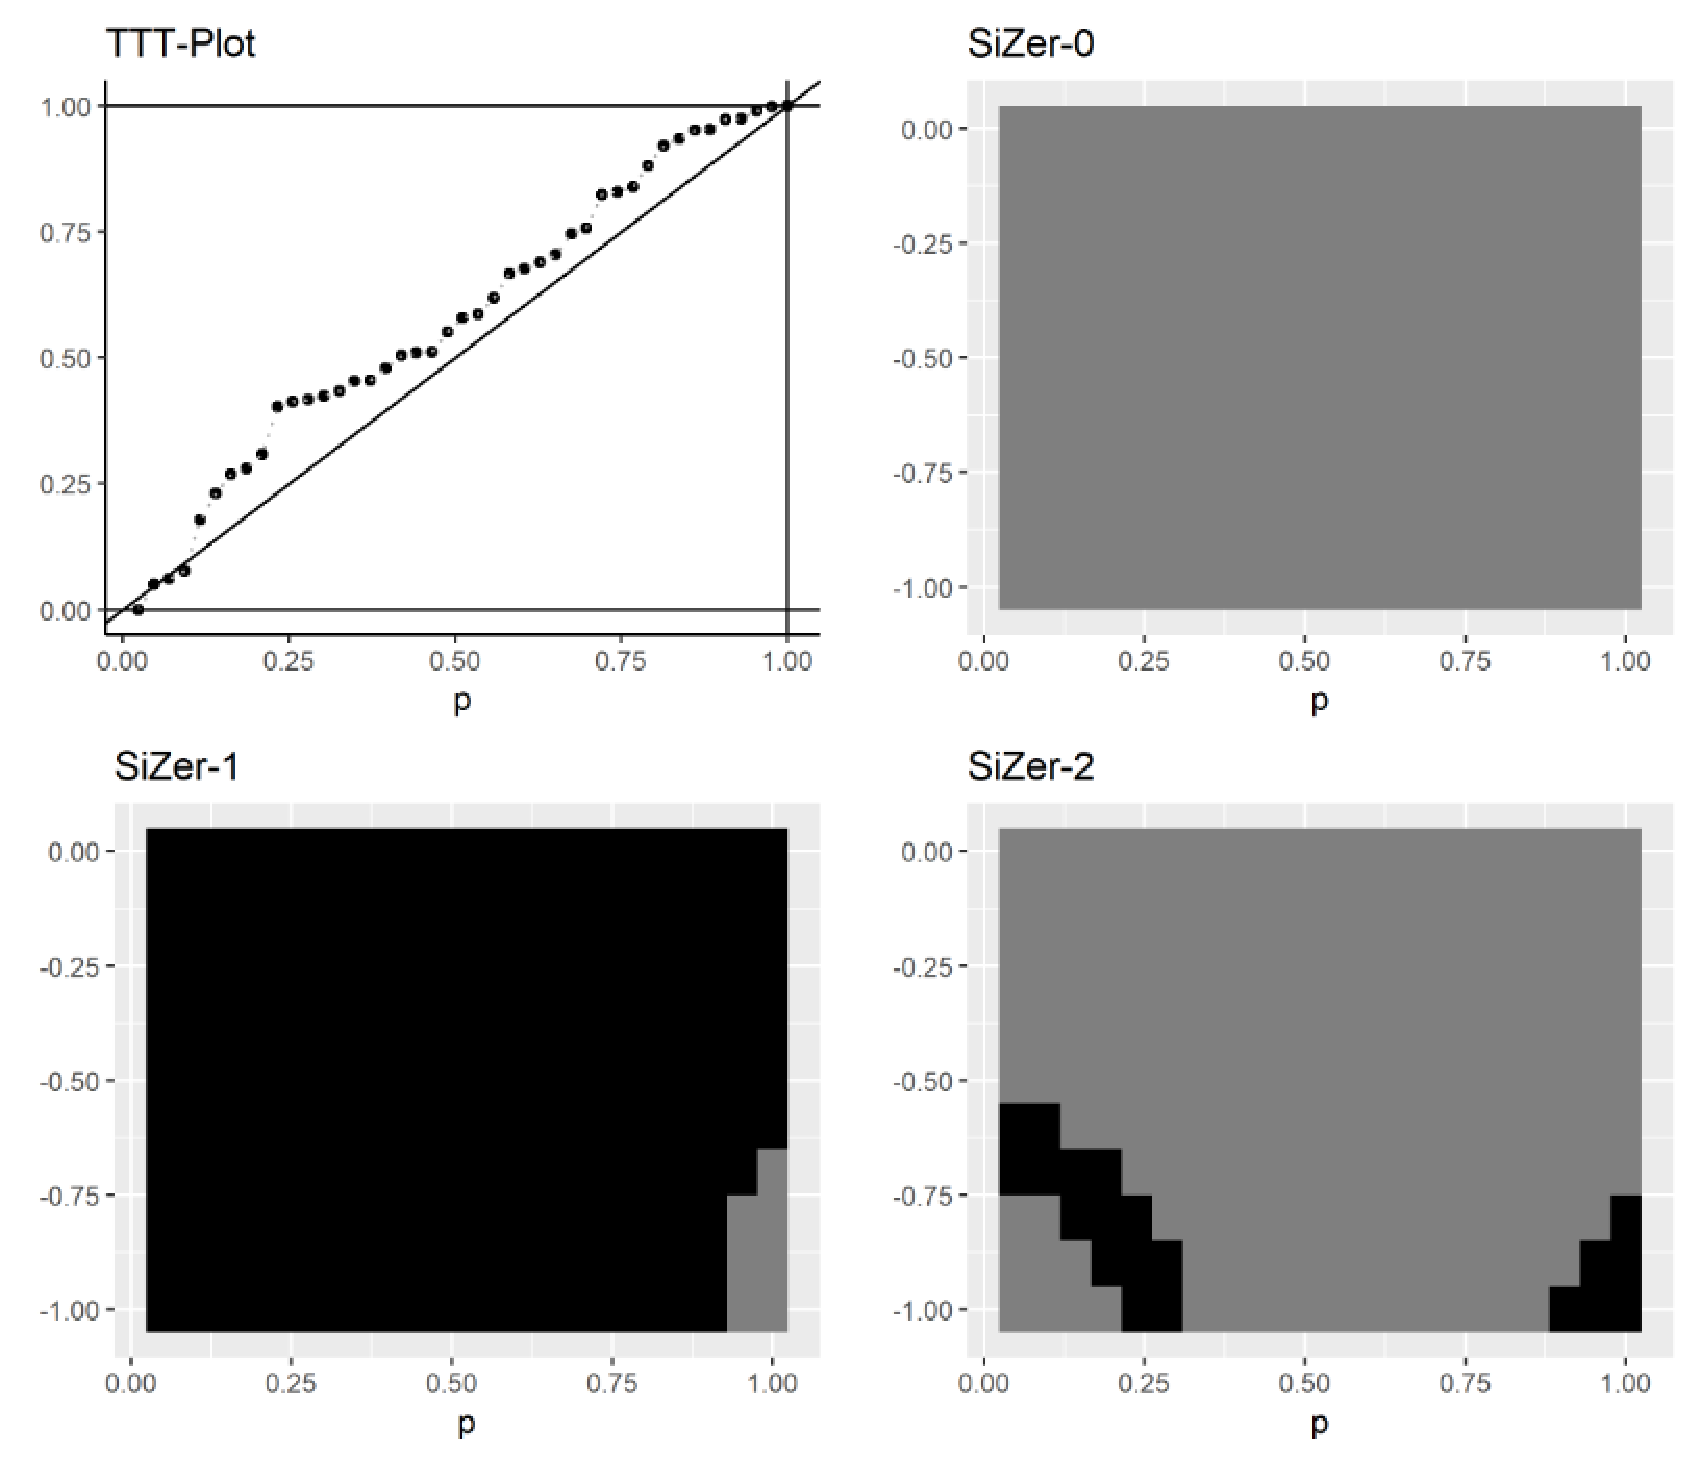
\includegraphics[height= 9cm]{Fig7_granulocyticQuadraticPuntual_01}%.EPS}
\caption{TTT-Sizer for Example 4: Survival days of chronic granulocytic leukemia.}\label{Fig:granu}
\end{center}
\end{figure}
%

%%%%%% END OF APPENDIX
%%%%%%%%%%%%%%%%%%%%%%%%%%%%%%%%%%%%%%%%%%%%%%%%%%%%%%%%%%%%%%%%%%%%%%%%%%%%%%%%%%%%
\begin{thebibliography}{}


\bibitem{BP75} Barlow, R. E. and Proschan, F. \textit{Statistical theory of reliability and life testing: Probability Models}. (1975) Holt, Rinehart and Winston.

\bibitem{RH04} Rausand, M., and Hoyland, A. \textit{System reliability theory: Models, Statistical Methods, and Applications}. Second edition (2004), John Wiley $\&$ Sons. 

\bibitem{KM2019} Khan, R.A. and Mitra, M. \textit{Sharp bounds for survival probability when ageing is non monotone}. Probability in the Engineering and Informational Sciences, 33, (2019) , pp. 205--219

\bibitem{KBM2020} Khan, R.A., Bhattacharyya, D. and Mitra, M. \textit{A change point estimation problem related to age replacement policies
}. Operations Research Letters, 48, (2020), pp. 105–-108.


\bibitem{Lillo00} Lillo, R.E. {\bf Note on relations between criteria for aging}. Reliability Engineering and System Safety, 67, (2000), pp. 129--133.

\bibitem{LX06} Lai, C.D., and Xie, M. {\it Stochastic aging and Dependence for Reliability}. (2006), Springer.


%

\bibitem{FPS2014} Franco-Pereira, A. and Shaked, M. \textbf{The total time on test transform and the decreasing percentile residual life aging notion}. Statistical Methodology, 18, (2014), pp. 32--40.

\bibitem{NASS2014} Navarro, J., Del Aguila, Y., Sordo, M.A. and Su\'arez-Llorens, A. {\bf Preservation of reliability classes under the formation of coherent systems.} Applied Stochastic Models in Business and Industry, 30, (2014), pp. 444-–454.


\bibitem{Sz2018b} Szymkowiak, M.  {\bf Generalized aging intensity functions}. Reliability Engineering and System Safety, 178(C), (2018), pp. 198--208.



\bibitem{NSB2013} Nair, N.U., Sankaran, P.G. and Balakrishnan, N. {\it Quantile-based reliability analysis}. (2013), Birkhauser.


\bibitem{Klefsjo82} Klefsjo, B. \textbf{On aging properties and total time on test transforms}. Scandinavian Journal of Statistics, 9, (1982), pp. 37--41.

\bibitem{NS2013} Nair, N.U. and Sankaran, P.G. \textbf{Some new applications of the total time on test transforms}. Statistical Methodology, 10 (1), (2013), pp. 93--102.


\bibitem{Klefsjo83a} Klefsjo, B. \textbf{Some tests against aging based on the total time on test transform}. Communications in Statistics - Theory and Methods, 12 (8), (1983), pp. 907--927.

\bibitem{A1987} Aarset, M.V. \textbf{How to identify a bathtub hazard rate}. IEEE Transactions on Reliability, 36 (1) (1987), pp. 106--108.


\bibitem{ZHMS2018} Zaretalab, A., Haghighi, H. S., Mansour, S., and Sajadieh, M.S. \textbf{A mathematical model for the joint optimization of machining conditions and tool replacement policy with stochastic tool life in the milling process}. The International Journal of Advanced Manufacturing Technology, 96, (2018), pp. 2319--2339.

\bibitem{LS2019} Lindqvist, B.H. and Samaniego, F.J. {\bf Some new results on the preservation of the NBUE and NWUE aging classes under the formation of coherent systems}. Naval Research Logistics, 66, (2019), pp. 430–-438.

\bibitem{KL98} Kvaloy, J.T. and Lindqvist, B.H. \textbf{TTT-based tests for trend in repairable systems data}. Reliability Engineering and System Safety, 60 (1), (1998), pp. 13--28.

\bibitem{VV09} Viertava, J. and  Vaurio, J.K. {\bf Testing statistical significance of trends in learning, aging and safety indicators}, Reliability Engineering and System Safety,  94, (2009), pp. 1128-–1132.

\bibitem{Anis2013} Anis, M. {\bf Tests of non-monotonic stochastic aging notions in reliability theory} Statistical papers, 55 (3) (2013), pp. 691--714.

\bibitem{SSA2018} Sreelakshmi, N. Sudheesh, K.K, and Asha, G. {\bf Quantile based tests for exponentiality against DMRQ and NBUE alternatives}. Journal of the Korean Statistical Society, 47 (2), (2018), pp. 185--200.

\bibitem{IM2019} Izadi, M., and Manesh, S.F. {\bf Testing exponentiality against a trend change in mean time to failure in age replacement}. Communications in Statistics -- Theory and Methods, (2019) DOI: 10.1080/03610926.2019.1702693.


\bibitem{CMO2019} Cuparic, M., Milosevic, B., and Obradovic, M. {\bf New $L^2$-type exponentiality tests}. SORT, 43 (1), ( 2019), pp. 1--26.



\bibitem{HE2000} Hutson, A.D. and Ernst, M. \textbf{The exact bootstrap mean and variance of an L-estimator}. Journal of the Royal Statistic Society, B. 62 (1), (2000), pp. 89--94.


\bibitem{CM99} Chaudhuri, P. and Marron, J.S. \textbf{SiZer for Exploration of Structures in Curves}. Journal of the American Statistical Association, 94 (447) (1999), pp. 807--823.

\bibitem{CM02} Chaudhuri, P. and Marron, J.S. \textbf{Curvatuve vs. Slope Inference for Features in Nonparametric Curve Estimates}. (2002) {\it Unpublished manuscript}.

\bibitem{PHK2009} Park, C., Hannig, J. and Kang, K.H. \textbf{Improved SiZer for time series}. Statistica Sinica, 19, (2009), pp. 1511--1530.

\bibitem{PK2008} Park, C. and Kang, K.H. \textbf{SiZer analysis for the comparison of regression curves}. Computational Statistics $\&$ Data Analysis, 52 (8), (2008), pp. 3954--3970. 


\bibitem{MU2004} Marron, J.S. and de U\~na \'Alvarez, J. \textbf{SiZer for length biased, censored density and hazard estimation}. Journal of Statistical Planning and Inference, 121 (1), (2004), pp. 149--161. 

\bibitem{PZ2007} Pittau, M.G. and Zelli, R. \textbf{Exploring patterns of income polarization using siZer}. Journal of Quantitative Economics, 5, (2007), pp. 101--111.


\bibitem{Setal2009} Sonderegger, D.L., Wang, H., Clements, W.H. and Noon, B.R. \textbf{Using SiZer to detect thresholds in ecological data}. Frontiers in Ecology and the Enviroment, 7, (2009), pp. 190--195.


\bibitem{P2005} Park, C., Hern\'andez-Campos, F., J. Marron, J.S. and Smith, F.D. \textbf{Long-range dependence in a changing Internet traffic mix}. Computer Networks, 48 (3), (2005), pp. 401--422.



\bibitem{Marron2020} Marron's Matlab Software - J.S. Marron (Steve Marron) . $http://marron.web.unc.edu/sample-page/marrons-matlab-software/$; 2020 $[accessed 17 February 2020]$


 
\bibitem{XieLai96} Xie, M. and Lai, C.D.  \textbf{Reliability analysis using and additive Weibull model with bathtub-shaped failure rate function}. Reliability Engineering and System Safety, 52 (1), (1996), pp. 87--93.



\bibitem{HM2006} Hannig, J. and Marron, J.S. \textbf{Advanced Distribution Theory for SiZer}. Journal of the American Statistical Association, 101 (474), (2006), pp. 484--499. 


\bibitem{NPY15} Novikov, A., Pusev, R. and Yakovlev, M. Package ''exptest´´. (2015) https://cran.r-project.org/web/packages/exptest/.


\bibitem{Ascher90} Ascher, S. \textbf{A survey of tests for exponentiality}. Communications in Statistics - Theory and Methods, 19 (5) (1990), pp. 1811--1825.



\bibitem{RMP07} Rondonotti, V., Marron, J.S., and Park, C. \textbf{SiZer for time series: A new approach to the analysis of trends}. Electronic Journal of Statistics, 1, (2007), pp. 268--289.



\bibitem{ABN08} Arnold, B.C., Balakrishnan, N. and Nagaraja, H.N. \textit{A First Course in Order Statistics. Classics in Applied Mathematics}. (2008) New York: Willey. 




%%%%%%%%%%%%%%%%%%%%%%%%%%%%%%%%%%%%%%%%%%%%%%%%%%%%%%%%%%%%%%%%%%%%%%%%%%%%%%%%%%%%



\end{thebibliography}
\end{document}
